\chapter{Methodology}
\label{ch:methodology}

\begin{quote}
    I can imagine no better place than a Northwestern logging camp for a philologist to spend a summer in. Here\ldots he can earn five dollars a day, breathe mountainy air, enjoy the keen smells of the conifers, and build up the abdominal muscles for chesty logger talk while he is making his investigations. \citep[139--140]{stevens_1925}
\end{quote}

In this chapter I discuss the methods for data collection, processing, and analysis that I use in this study.\footnote{The procedures for recruitment, consent, and data analysis described in this chapter were approved by the Univeristy of Georgia Institutional Review Board on April 11, 2016. The study ID is STUDY\liningnums{00003041}.} I begin by describing my fieldwork methods in \S\ref{fieldwork}, including how participants were recruited, the interview itself, and the equipment used for recording. Next, in \S\ref{participant_metadata}, I describe the demographic metadata about the participants and provide a brief description of the participants in this study. I discuss how my data was transformed from raw audio files to spreadsheets of numbers in \S\ref{processing}, including transcription, forced alignment, formant extraction, and filtering. Then, I use \S\ref{word_classes} to explain the word classes in this study, including their labels and how they are defined. In \S\ref{corpus_size_constitution}, I describe the corpus size and constitution. Finally, I discuss the statistical analysis for this study in \S\ref{statistical_analysis}. In summary, this dissertation uses traditional techniques for data collection, standard procedures for processing, and recent developments in statistical modeling for analysis.

% --------------------------------------------------------------------
% ------------------------    Fieldwork    ---------------------------
% --------------------------------------------------------------------

\section{Fieldwork}
\label{fieldwork}

The data analyzed in this study was collected via sociolinguistic interviews. This technique is an adaption of the traditional dialectology interviews of the early 20th Century in that participants participated in a guided conversation while being recorded. However, rather than being focused on eliciting key linguistic items, the sociolinguistic interview aims to collect speech samples in a variety of styles, from casual discourse to situations where speakers pay the most attention to speech. This method is subject to some criticism (see, for example, \citealt{wolfson_1976}), but it continues to be the standard and most popular method for data collection in sociolinguistics.

\subsection{Participant recruitment}

I collected the data that is used in this dissertation during late June and most of July 2016 in Cowlitz County, Washington. Participants were recruited primarily through my family’s contacts, but I also timed the trip so that I could find potential participants at the Go Fourth Festival, an annual celebration at Lake Sacajawea around the 4th of July, and contact local organizations like the high school’s alumni association. A few participants were recruited through social media and others face-to-face, especially on the campus of Lower Columbia College in Longview. Those who were interviewed were also invited to participate in the recruitment process themselves through word of mouth or, especially in the second half of the trip, through specially designed business cards. In total, I interviewed fifty-four self-described natives of Cowlitz County, loosely defined as being born in or having spent most of their life in the area.

\subsection{The sociolinguistic interview}

The primary goal when meeting participants was to make the environment as casual and comfortable as possible. The interviews occurred at places convenient for the interviewees such as speakers’ homes (living rooms or kitchen tables), churches, and offices or in public places like a conference room in the Longview library, the student center at Lower Columbia College, and a Starbucks. Following \citet{feagin_2013}, I dressed appropriately for the age of the participants by wearing casual clothes for younger people and business casual for older participants.\footnote{\citet[37]{hall_lew_2009_diss} mentions that she made the effort to dress as consistently as possible for all the interviews, which made her more easily recognizable at community events. I felt that modifying my dress for the interviewer, particularly for the older people, was more appropriate in this community.} Because of the power asymmetry that may be present when meeting an ``expert'' researcher \citep[197]{schlling_2013}, I emphasized my status as ``just a student'', both in conversation and appearance. Specifically, I looked the part by wearing a backpack and kept my ``nothing special'' equipment\footnote{As described below, the equipment was good, but I downplayed it a little bit in front of the participants.} in a handmade bag. Additionally, I frequently mentioned my wife and newborn child to show that I was a regular person. However, I ``temporarily step[ped] into the `expert' role'' \citep[236]{schlling_2013} when presenting the consent forms and setting up recording equipment to convey to the participants that the recordings would be of good quality and that I would treat them with great care. At each location, I made efforts to reduce background noise by turning off fans, air conditioning units, ticking clocks, and, in one case, a particularly noisy refrigerator.

For roughly half of the interviews, my mother-in-law was present and played an active role as an interviewer. \citet[110]{schlling_2013} points out that it may seem counterintuitive to introduce a second interviewer because it may swing the power dynamic too far towards the interviewers; however a third person in the room eliminates the potentially uncomfortable one-on-one setting, making the interview feel more like a conversation and less like an interrogation. In the case of my mother-in-law, while she is not a native of Cowlitz County, she has lived there for over 20 years and has achieved an in-group status that I could have never obtained as a visiting researcher. Plus, she is a great conversationalist and did an exceptionally good job at getting people to talk. In other words, introducing a third party to the interviews allowed participants to be more relaxed, allowing for more natural discourse.

The format of the recording session was that of a traditional sociolinguistic interview \citep{labov_1984}. After greetings and introductions, participants signed consent forms and were briefed on the purpose of the study, though specific linguistic features were not mentioned. After consent was given, the microphone was turned on and a 35--50-minute conversation followed.\footnote{Most interviews started with something along the lines of, ``The purpose of this is to get you talking as much as possible, so feel free to go off on tangents and tell the `long version' of stories. Basically, just tell me your life story. You have 45 minutes. Go!'' I initially started this way half-jokingly, but it actually turned out to be an effective way to get people to start talking.} Conversation topics were modified from recommended questions and protocols used by \citet{wolfram_1974}, \citet{tagliamonte_2006}, and Labov \citep{labov_1998_2004, labov_1984}. However, they were supplemented to include questions that would be more relevant to this particular community, such as asking about Portland, Seattle, the mills, and local natural disasters. By far the best question was to ask about experiences related to the eruption of Mount St. Helens in 1980, which turned out to be the most effective tool for eliciting narrative and natural discourse in this community (cf. \citealt[92]{moonwomon_1991_diss} on eliciting stories about a recent earthquake in her work in San Francisco). Few participants were in any danger, but most were excited to tell their stories. Even some of the younger speakers were happy to relate their parents' stories. When the prepared questions failed to pique the informants' interests, the topic of conversation turned to their hobbies and other interests. In all cases, the interviewers spoke relatively little, and the bulk of the conversation was taken up by the informants' speech.

At the end of the conversation, participants were asked to complete several tasks in order to elicit a more careful speech style (see Appendix~\ref{appendix:reading_passages}). First, participants read a short, neutral, three-sentence passage called ``Friends'' to evaluate their reading level and comfort.\footnote{The passage was used by Labov in New York and did not target any specific features in either of our studies \citep[417]{labov_2006}.} If there were no perceived difficulties (i.e. illiteracy or vision-impairment) and if time permitted, participants were asked to read a longer passage called ``The Cat and the Mice'' \citep{freeman_2014}. This adaptation of one of Aesop's Fables was written by Alicia Wassink to specifically target features known to be variable in Washington. The subject matter of this passage was entertaining enough that participants rarely made any comment about specific words it contained, suggesting that they were likely not aware of the particular linguistic variables being studied.

To move on to an even more careful speech style, one that is used when all context is stripped out and focused on individual words, speakers then read a 160-item word list. This list was carefully crafted to elicit multiple tokens of variables that are known to currently be in flux in the Pacific Northwest (pre-velar raising, back vowel fronting, the low back merger), variables that were mentioned in \textit{Linguistic Atlas of the Pacific Northwest} but have not received as much attention in contemporary research (the \textit{hoarse-horse} merger,\footnote{Most North American English speakers merge \north with \force (\textit{i.e.} the \textit{hoarse-horse} merger), but in a few scattered dialects, the distinction between the two may be retained or \north may be merged with \start (\textit{i.e.} the \textit{cord-card} merger) \citep{labov_ash_boberg_2006_anae}. \citet[560]{reed_1961} suggests that some speakers in the Pacific Northwest do not have the \textit{hoarse-horse} merger and instead have some other configuration. None of the speakers in this sample appeared to have anything but the mainstream \textit{hoarse-horse} merger.} the \textit{Mary-merry-marry} merger, /r/-intrusion in \textit{wash}, (wh)-aspiration, and palatalization of words like \textit{dew} and \textit{Tuesday}), and a few variables not known to be variable in the region like low and back vowels before laterals \citep[cf.][]{stanley_2017_ADS} and (thr)-flapping \citep[cf.][]{stanley_forthcoming_thr}. The words were randomized and then the order was manually adjusted where needed so that that adjacent words did not contain the same vowel. Visually, the words were displayed in a four-by-four grid, with each cell containing 10 tokens in one column, center-aligned (see Apppendix~\ref{appendix:wordlist}). Most participants read the words from top to bottom, left to right while a few read the words left to right, top to bottom. Because the list was presented as ``just a list of random words,'' participants did not appear to catch on to the specific linguistic variables or to the fact that it was an unbalanced sample of English (there were no high front vowels, and a disproportionate number of pre-lateral tokens).

After the wordlist, speakers were asked complete a minimal pair task to focus their attention on individual sounds (see Apppendix~\ref{appendix:minimal_pairs}). The list of 40 pairs and 5 minimal triplets were again carefully selected following similar criteria as the word list, except the targeted variables were potential mergers only. In addition to production data, this task elicited some intuition of the vowel classes in question: speakers were asked after each minimal pair and triplet to say whether they thought they pronounce the words the same. There were at least two pairs of words that targeted each possible merger (sometimes as a part of a minimal triplet), providing a small indication of the degree to which the pair is merged for an individual. To test speakers’ attention (since this was the final task after an hour of talking) the list included a few filler pairs are presumably homophonous for all North American English speakers (e.g. \textit{stairs} and \textit{stares}).

In some of the interviews, participants were asked to also take part in an “elicitations” task where I would ask questions that would prompt them to say specific words. The following list displays the questions that I asked with the intended token in italics.
\begin{enumerate}
    \item Could you count for me from 1 to 10? \textit{two}, \textit{six}, \textit{seven}, \textit{ten}
    \item And would you please say the days of the week? \textit{Tuesday}, \textit{Wednesday}, \textit{Saturday}
    \item Can you list as many articles of clothing as you can think of? \textit{pants}, \textit{coat}, \textit{hat}, \textit{cap}, \textit{boots}
    \item What sorts of things would people make for breakfast on a holiday or if they had family over? \textit{eggs}, \textit{toast}, \textit{juice}, \textit{coffee}, \textit{hash browns}
    \item What kinds of spices would you find in someone’s cupboard? \textit{nutmeg}, \textit{oregano}, \textit{cinnamon}
    \item What kinds of animals would you see on a farm? \textit{goat}, \textit{dog}, \textit{horse}
\end{enumerate}
This task actually proved quite effective in eliciting specific tokens in certain vowel classes. For example, there were several tokens of back vowels (\textit{two}, \textit{Tuesday}, \textit{boots}, \textit{juice}, \textit{coat}, \textit{toast}, \textit{goat}), low back vowels (\textit{dog}, \textit{coffee}), prevelars (\textit{eggs}, \textit{nutmeg}, \textit{oregano}), prenasal tokens (\textit{cinnamon}, \textit{ten}, \textit{Wednesday}, \textit{pants}), front lax vowels (\textit{six}, \textit{seven}, \textit{Saturday}, \textit{hash browns}, \textit{cap}, \textit{hat}), and a token of \north (\textit{horse}). However, I forgot to do the task for all speakers, so this data was inconsistent across the corpus. For the purposes of this study, these elicited tokens will be grouped with the conversation data.

\subsection{Equipment}

The equipment for the interviews was of sufficient enough quality for sociophonetic analysis. Most participants wore a JK MIC-J 044 lavalier microphone, positioned about a foot away from their mouths and slightly to the side, connected to a TASCAM DR-05 digital recorder at 48kHz sampling rate and 24-bit depth. Because of technical difficulties, two interviews were recorded on backup equipment:\footnote{These were used for the fourth and fifth interviews (Megan and Brandon), because the SD card in the handheld recorder was full after the first four interviews and I hadn’t yet figured out how to transfer the files to my laptop.} a Blue Yeti microphone connected to an early 2013 model MacBook Air, using Praat \citep{boersma_weenink_2018_praat} as the recording software with similar audio specifications. Interviews were recorded in WAV format and stored on a shock-resistant external hard drive dedicated to the project. No problems occurred with the equipment and no data was lost during or since fieldwork.


% --------------------------------------------------------------------
% -------------------    Participant Metadata    ---------------------
% --------------------------------------------------------------------

\section{Participant metadata}
\label{participant_metadata}

I chose to gather speaker metadata using indirect means. In other words, participants were not asked directly about their age, gender, ethnicity, socioeconomic status, or any other demographic information. However, some of this information was offered freely during the interview. For example, some participants disclosed their age or birth date during introductions at the beginning of the interview. Most others gave indirect clues, such as mentioning offhand the year they graduated from high school or how old they were during the eruption of Mount St. Helens. Together with my personal judgments, these indirect clues were used to code age and sex for each participant.

For the purposes of this study, age was treated as a categorical variable. One reason is because while the age range in this sample was relatively wide (ranging from 18 to 86 at the time of interview), it was patchy and unbalanced across the sexes. This sample made it difficult to model nonlinear language change\footnote{See \S\ref{gamms_in_this_study} for details.} and I did not want to assume that change occurs at a constant rate across the time span represented by this corpus. Another reason is that the very oldest speakers were all men and the youngest were all women and I did not want this pattern to affect the results. Furthermore, in \citet{stanley_2018_pwpl}, I show that catastrophic language change occurred in this community, resulting in large differences between generations but no significant change within them. This suggests that at least some language change occurs stepwise rather than linearly in this community, so a categorical approach may be a more appropriate model.

To define the age categories, I grouped speakers by nationally recognized generational cohorts \citet[cf.][]{donofrio_etal_2019}. The Pew Research Center defines four generations as the Silent Generation (born 1928–1945), Baby Boomers (born 1946–1964), Generation X (born 1965–1980), and Millennials (born 1981–1996).\footnote{See \citep{strauss_howe_1991} for much more detail on these and older generations.} Coincidentally, the boundaries between these generation correspond to natural gaps in the sample under study. Figure 1.1
\sidenotetext[\vspace{0em}]{ %had to put some marker or else it would default to footnote 9. This hspace works
    \footnotesize
    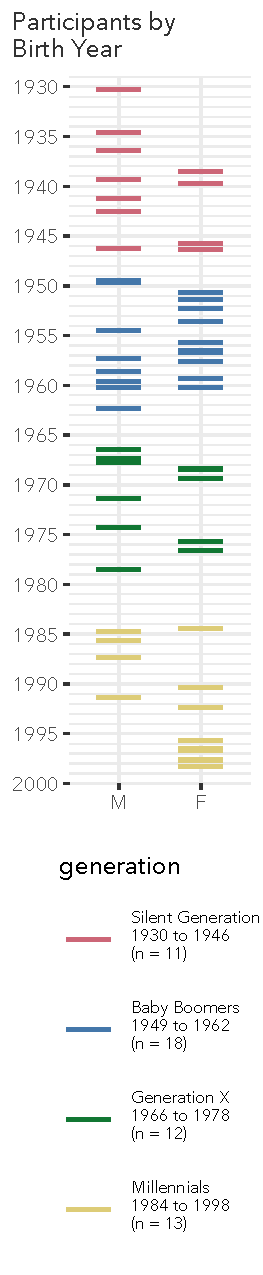
\includegraphics[width = 1.6in]{Figures/methods/age_tall.pdf}
    Figure 1.1: Age distribution by sex of the participants in this study. Some jitter has been added to view overlapping speakers.
}\addtocounter{figure}{1} % Since I manually put this figure, I'll increment the figure count.
shows the 54 speakers' birth years, divided by sex and colored by generation. There were no speakers born in 1963–1965, forming a break that happens to be around the time the Baby Boomer generation ends and Generation X begins. Furthermore, there were no speakers born 1979–1983, which was the tail end of Generation X and the beginning of the Millennials. This also corresponds to a crucial time period in Cowlitz County when the timber industry was undergoing major changes and the community was in a deep recession, as described in detail in \S\ref{sec:rise_and_fall}.

%\begin{figure*}[htb]
%    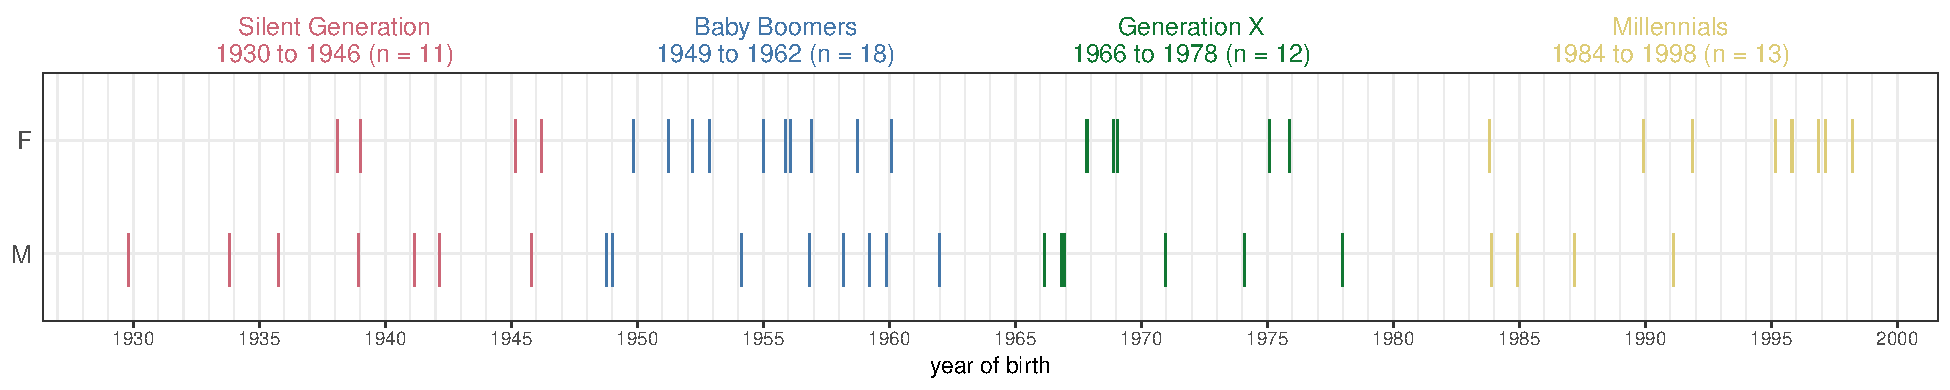
\includegraphics[width = 6.5in]{Figures/methods/age.pdf}
%    \caption[Years of birth and generations by sex.]{Years of birth and generations by sex. A small amount of jitter has been added to the birth years to allow for the viewing of multiple speakers of the same sex and the same birth year.}
%    \label{fig:age}
%\end{figure*}

There are two very small modifications to the generations defined by the Pew Research Center and the generations that will be used in the present study. First, 1946 is normally considered the first year of the Baby Boomer generation, but I felt that the two participants born in that year, Earl and Elizabeth, fit in culturally more with the Silent Generation than with the rest of the Boomers. Also, the Pew Research Center \citep{dimock_2018} has recently defined 1996 as the last year of the Millennial generation, and all those born in 1997 or later will be part of the next generation (which has not received an official name, though \textit{Generation Z} and \textit{Post-Millennial} are in circulation). In this sample, the three youngest speakers would fall into this cohort. However, it made little sense to classify those three as a separate generation, so they will be grouped with the Millennials. With these small changes in mind, these nationally recognized generational cohorts will be used as a placeholder for age in the analysis for this study.

For other demographic information, I grouped participants into broad categories. I assigned speakers binary sex based on their outward appearance. Only two participants brought up their ethnicity (one woman was half-Hispanic and another had Native American heritage); I judged all others to be Caucasian American, which is mostly what would be expected for Cowlitz County\footnote{A more complete description the demographics of Cowlitz County is provided in \S\ref{sec:physical_description}, but according to the 2017 population estimates, the county was 83.7\% White (not Hispanic or Latino) \citep{census}. In other words, I oversampled the White population with respect to the actual population.}. For the purposes of this dissertation, sexual orientation is not considered for analysis as it was rarely brought up by any of the participants, the exception being one person who self-identified as a homosexual man. Incidentally, nearly every participant who I judged to be male mentioned a wife or girlfriend and those who I judged to be female mentioned husband or boyfriend. This subjective and oversimplified classification of sex, gender, ethnicity, and sexual orientation admittedly glosses over the nuances in these features of a person's identity; future work in Cowlitz County is needed to see the effects that these factors have on language.

Each participant was assigned a pseudonym. Following \citeauthor{tagliamonte_2006} (\citeyear[51]{tagliamonte_2006}, cf. \citealt[253--254]{schlling_2013}), I refer to speakers in this dissertation by alternative names rather than numbers because they are easier to remember and give more life to their excepts. I selected names based on the person’s age and chose a name that was common during their year of birth as their pseudonym.\footnote{See Table~\ref{tab:speaker_summary} below for the list of names.}



% --------------------------------------------------------------------
% ------------------------    Processing    --------------------------
% --------------------------------------------------------------------

\section{Processing}
\label{processing}

After the interviews were completed, there are several steps of processing required to produce data in a format ready for quantitative analysis. In this section I describe the methods for transcription, forced alignment, formant extraction, and filtering, normalization, and Bark-transformation that I used in this study.

\subsection{Transcription}
\label{transcription}

The first step in data processing was to transcribe the audio. There exists software and hardware designed to facilitate transcription, but I found it easiest to simply do it manually in Praat \citep{boersma_weenink_2018_praat} for several reasons. First, after doing some preliminary tests with automatic speech-to-text software, such as the one as part of the DARLA suite \citep{reddy_stanford_2015_DARLA}, I found that it took longer to correct these transcriptions than it would have to just transcribe it myself. Second, I was most comfortable in Praat than in some other software like ELAN or Transcriber and felt like I could create more accurate boundaries to the utterance phrases than I could using other programs, given my skills in them. Finally, I wanted the output to be in Praat’s TextGrid format because I intended to use Praat scripting to extract information from the corpus, and eliminating a middle man seemed the most efficient.

I developed and adhered to some basic protocols while transcribing. I used standard English spelling with the exception of a few words like \textit{gonna}, \textit{wanna}, and \textit{cuz} (``because''). All speech was transcribed at the utterance-level regardless of syntactic boundaries. In fact, I did not attempt to parse the syntactic structure of the speech at all, so intervals were treated as continuous strings of words without regard to when prosodic phrases started or ended. Capitalization at the beginning of utterances was ignored, but it was retained in proper nouns and the pronoun \textit{I}. I likewise did not include punctuation except for apostrophes (in both contractions and possessives, which are required to distinguish words like \textit{well} and \textit{we'll}) and hyphens. All intelligible speech by the participants was transcribed, including stutters and other speech errors if an entire word was uttered. Other types of disfluencies, partially uttered words, and other noise (lip smacks, coughs, laughter) were left blank so that the forced aligner would skip over them. Interviewer speech was not transcribed; neither was speech that overlapped with the interviewers. It took 174 hours to transcribe the approximately 41 and a half hours in the conversation portion of the corpus (a rate of approximately 4.2 hours to transcribe one hour of audio).\footnote{The conversation portion of the corpus was transcribed in two waves. I did the first third April--August 2017. The remaining two-thirds were completed between April and July 2018.}

\subsection{Forced alignment}
\label{forced_alignment}

For this project, I used a local installation of the Montreal Forced Aligner \citep{macauliffe_etal_2017_MFA} to process the conversation portions of the transcribed audio. I chose this tool over other forced aligners for two reasons. First, it is relatively new and is built with Kaldi \citep{povey_etal_2011_kaldi}, which is being actively maintained and developed. Second, having the software on my own machine (as opposed to an online-based aligner like DARLA or WebMAUS) was appealing and convenient. The aligner also checks for out-of-dictionary words which facilitates the identification of typos and other misspellings, which I manually corrected. The dictionary for this aligner was the LibriSpeech corpus which will be discussed in the next section.

One of the benefits of the Montreal Forced Aligner is that it implements a speaker-level adaption in alignment. Before processing the audio, it measures acoustic properties about the speaker’s voice which it then uses to fine-tune the built-in acoustic model. However, the aligner had trouble processing the interview files because of their length, so as part of the pre-processing stage, a Praat script was written to split the audio and transcription files in half. These two halves were processed separately, though not independently. By this, I mean that the aligner was made aware that both halves came from the same speaker so the acoustic model was trained using all the speaker’s data rather than processing each half independently from the other.

Because the reading portions of the corpus were transcribed much earlier, they were processed differently. They, too, were transcribed by hand, but they were force-aligned using the DARLA suite \citep{reddy_stanford_2015_DARLA}, which, at that time, used ProsodyLab-Aligner \citep{gorman_etal_2011_prosodylab} for this task. The alignments for all segments in the word list and minimal pair tasks were hand-checked for accuracy and corrected where needed. The output of the conversation portion of the corpus was not hand-corrected, but \citet{strelluf_2019} has shown that manual correction of vowel boundaries has little effect on the results when they are presented in a summarized format, which is how they are presented in this study.

\subsection{Formant extraction}
\label{formant_extraction}

Humans use many cues from the speech signal for processing vowel sounds. Because they reflect the shape of the vocal tract, ``formants of a sound are properties of the corresponding mouth shape'' \citep[98]{ladefoged_1996}. But \citet{dipaolo_faber_1990} illustrate the need for additional acoustic variables in their analysis of what appears to be the loss of a tense-lax distinction before laterals (the \textit{feel-fill}, \textit{fail-fell}, and \textit{pool-pull} mergers) in Salt Lake City, Utah. While the vowel classes occupy the same in the F1-F2 vowel space, the laryngeal configurations of the vocal tract were used to reliably distinguish the vowel classes. Putting it succinctly, ``there is more to vowels than their formant frequencies'' \citep[201]{dipaolo_faber_1990}. Though they are not a focus of this dissertation, the multidimensional nature of speech sounds is especially true of consonants too: the distinction between what are traditionally called ``voiced'' and ``voiceless'' consonants in English can differ by as many as 16 dimensions \citep{lisker_1986}. What kind of variation is possible in these other facets of speech sounds, and what kind of social meaning can be associated with their variants?

It is out of the scope of this study to include many aspects of the speech signal in my analysis, but there is a need for other acoustic measurements in the study of the Elsewhere Shift. Because of the inconsistencies between studies that focus on these vowel changes, \citet[150]{boberg_2005} wonders whether there's more to the shift than F1 and F2. While this study will continue the trend by only using F1 and F2 measurements for analysis, I do expand my sampling of the vowel to more than just one point along its duration. \citeauthor{jacewicz_etal_2006} analyzed their data twice, once looking at midpoints alone and again looking at formants extracted at five time points, and find that ``dialect differences could well exist but remain unnoticed as a result of the less robust methodology traditionally used'' \citeyearpar[300]{jacewicz_etal_2006}. One goal for this dissertation is to show how the speech in Cowlitz County compares to other areas with the Elsewhere Shift, and the best way to maximize this comparison is to use similar methods as previous studies. For this reason, I limit my analysis to vowel formants alone, and hope that future work will describe the shift in more phonetic detail.

Once the files were transcribed and aligned, the next step in the process is to extract formant measurements from the speakers’ vowels. I chose to do this using a Praat script rather than using software such as FAVE-Extract \citep{rosenfelder_etal_2014} to allow for more flexibility in the output. In its current implementation, FAVE extracts formant measurements at five points along the duration of the vowel. While this is sufficient to analyze the trajectory of the vowel \citep{renwick_stanley_2020}, a more detailed view of these dynamic properties is possible when more data is extracted per vowel token. It is possible to modify FAVE to extract any number of tokens per vowel \citep[cf.][]{warburton_2018}, but I have found that this results in duplicate measurements across multiple time points, which is an undesirable result.

The script that I used for formant extraction was one that I wrote in Praat. Similar to the Montreal Forced Aligner, the software had difficulty processing the entire interviews at once, so the script first split the file into more manageable chunks that were approximately five-minutes long, ensuring that the split did not interrupt the informants' speech. For each vowel, measurements were taken at 11 equidistant points along its duration (onset, 10\%, 20\%, \ldots, 90\%, offset). I processed the audio four times, each using a different combination of settings in Praat. I altered the number of formants Praat should look for and the maximum Hz to consider when looking for those formants. The four combinations of settings were 5 formants with a maximum of 4500Hz, 5000Hz, and 5500Hz and 6 formants with a maximum of 5500Hz. This resulted in four versions of the data for each speaker, each produced slightly different settings and resulting in slightly different formant measurements.

The reason for this apparent redundancy was because a single combination of settings usually does not produce the cleanest results from the entire audio corpus. I had men and women in this sample with relatively high and low voices, so even different settings based on the sex of the speaker was not adequate. FAVE handles this issue by extracting four sets of measurements per token and selects the best based on distances from hand-checked measurements \citep[34--36]{labov_etal_2013}. My initial goal was to extract data using many more settings and use what I call the ``mistplot'' technique (\citealt{stanley_2018_mistplots}; see also \citealt{kendall_vaughn_2015}) to determine the best measurements, but constraints on time and computational power prohibited me from using this method in this project. Instead, to determine the best measurements, I simply plotted all data in the F1-F2 space and selected the set that appeared the cleanest per speaker, meaning I chose the setting that produced the fewest obvious gross outliers. For women, the most common setting was using five formants and 5000Hz, with the exception of six women (they all had relatively higher voices) whose best setting was 6000Hz. For the men, the most common setting was five formants and 5000Hz except for the three men whose voices were relatively higher voices and 5500Hz yielded cleaner results. There is admittedly some subjectivity in this selection technique, but I feel that the results were cleaner than applying the same settings for all speakers of the same sex.

\subsection{Filtering}
\label{filtering}

It is out of the scope of this dissertation to analyze all tokens of all vowels. I filtered out vowels that did not have primary lexical stress. I also removed diphthongs (\price, \mouth, and \choice) and syllabic /\textipa{\textrhookschwa}/ (\nurse). Finally, I excluded words if they were part of a 181-item list of stop words (see Appendix~\ref{appendix:stopwords}). Here, stop words were defined as words that are high frequency (including discourse markers like \textit{yeah} and \textit{y'know}), many of which were members of a closed class lexical category in English like pronouns and conjunctions.

Automatic methods in forced alignment and formant extraction save time, make it easier to process larger corpora, and are more objective than manual work; however, they come at the expense of data cleanliness. Manual checking and correcting of outliers was not done in this study, largely due to the size of the corpus. Tens of thousands of vowel tokens, each contributing 22 formant measurements (two formants at 11 time points), was judged to be too large to check by hand. As such, a method for filtering the data was necessary to exclude out the inevitable outliers in the data that are present because of software errors.

One of the most common methods for automatic detection and exclusion of outliers is to remove observations that have F1 or F2 measurements more than two standard deviations from the mean (a \textit{z}-score method). I argue that this method is inherently flawed because of the unnaturally rectangular distribution it produces. F1 and F2 represent height and backness axes, respectively, but tokens of the same vowel phoneme often fall along distributions that are diagonal to these dimensions. When F1 and F2 are correlated like this, bad tokens may fall within the normal range of formant values but they are still considered good data. Meanwhile, good data on the extremities of the distribution may be excluded.

Another method for detecting outliers is to calculate the Mahalanobis distance from each token to that vowel’s mean in a multivariate space \citep{mahalanobis_1936, renwick_ladd_2016, labov_etal_2013, evanini_2009_diss}. This method considers the distribution and correlation between the F1 and F2 measurements such that observations that a human would spot as outliers are often detected as such. Visually, this can be thought of as fitting an ellipse of some size to the data, centered around the mean, and anything outside of that ellipse is considered an outlier.

\begin{figure*}[tb]
    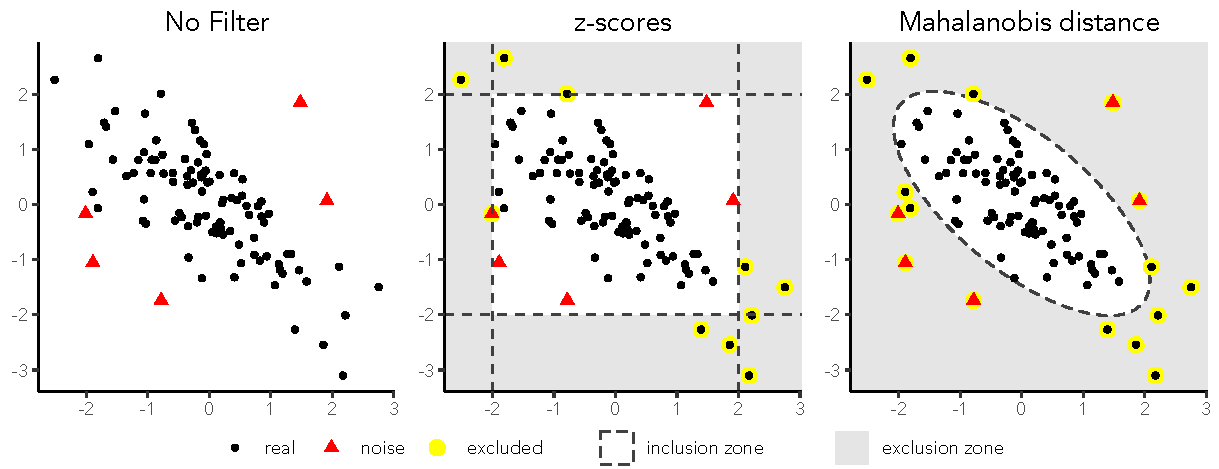
\includegraphics[width = 6.5in]{Figures/methods/filtering.pdf}
    \caption[A comparison of filtering methods]{A comparison of filtering methods on simulated data.}
    \label{fig:filtering}
\end{figure*}

Figure~\ref{fig:filtering} compares these two methods. For this plot, I generated 100 points based on a multivariate normal distribution and then added five points known to be outliers. The generated observations are plotted as black circles and the outliers as red triangles. This data is seen in the left panel of Figure~\ref{fig:filtering} and it is evident that though the outliers have F1 and F2 measurements that fit in with the rest of the data, it is the combination of their measurements (i.e. high F1 and F2 or low F1 and F2) that place them in areas relatively far from other data points. In the center panel, I apply a filter that excludes tokens if their F1 or F2 measurements are further than two standard deviations from the mean. These cutoff values are represented by the dashed lines and observations that fall outside of the square are highlighted in yellow. This center panel shows that none of the known outliers were excluded, but eight of the good points were. Another way of think about this technique is that it essentially fits a square cookie cutter to an ellipsoidal distribution. On the contrary, the right panel in Figure~\ref{fig:filtering} illustrates the filter based on the Mahalanobis distance. The dotted line in this panel encircles the area where the square root of the Mahalanobis distance is less than two, roughly corresponding to two standard deviations from the mean. Since this simulated data is ellipsoidal, the oval-shaped “cookie cutter” does a better job, and it excludes all of the known outliers. However, it is still not a perfect method because eight good data points were also excluded (mostly matching the eight removed in the center panel).

For this study, I chose to use the Mahalanobis distance as a way to detect potential outliers. For each vowel for each speaker, after the measurements from all time points were pooled together and were arranged by their multidimensional distance (in the F1-F2 space) from the mean, I did a blanket exclusion of the furthest 5\% of the tokens, which roughly corresponds to removing observations if the square root of their Mahalanobis distance is greater than two.

The use of the Mahalanobis distance is not without its flaws. Statistically, this method is sensitive to outliers because it relies on vowel means. The presence of many gross outliers can skew the distribution, causing the mean to be pulled to an unexpected position in the vowel space. When the mean is far enough from the ``true'' center of the distribution, good measurements may fall far enough from it that they get removed by the filter.\footnote{In \citet{stanley_2018_mistplots} I presented a preliminary modified version of the Mahalanobis distance for outlier detection that is less sensitive to outliers. For more information, see the \texttt{joeyr} package \citep{joey_2020_joeyr}. Due to limitations of computational power and time constraints, this technique was not implemented in this study. } The other flaw in the Mahalanobis filter is that it assumes that vowel data is multivariate normally distributed. \citet{vanhofwegen_2017_diss} has shown that this is not the case because speakers can make use of stylistic variants that cluster at the extremes of the distribution of the vowel tokens in other situations. To my knowledge, there is no best method for detecting and excluding potential outliers in sociophonetic data, but using the Mahalanobis distance method seems more theoretically-grounded and more appropriate---or at least less bad---than using standard deviations of F1 and F2 measurements.


\subsection{Normalization}
\label{normalization}

Because of physiological differences in humans, there is considerable variation in the formant measurements between speakers. Women and people with shorter vocal tracts tend to have higher formants and a larger overall vowel space while men and people with longer vocal tracts have lower formants. For computational processing, these differences are problematic when two people pronounce a vowel, because though a human would perceive the two to be the ``same,'' the formant values between two pronunciations may be quite different. For this reason, some sort of normalization procedure is desirable to allow for meaningful comparisons between speakers.

There is a myriad of normalization procedures in circulation today. A detailed account of how they are calculated and how well they appear to work is out of the scope of this dissertation, though \citet{adank_etal_2004} and the methods page of the \textit{NORM} suite \citep{thomas_kendall_2007_NORM} are good resources for this information. Recently, \citet{barreda_2019} has shown that the \citet{lobanov_1971} transformation is inherently flawed because it operates on F1 and F2 independently, is too powerful, and aims at a goal that is theoretically unsound. Instead, he advocates for some sort of log-mean-based method which applies a single metric to both F1 and F2 and is empirically well-supported. He does not claim that a log-based method is ``correct,'' but rather that it is less bad than the Lobanov transformation.

In this study, I use the log-mean normalization method adopted by the \textit{Atlas of North American English}. Their method, which is based on the one established by \citet{nearey_1978_diss}\footnote{See \citet[519 note 2]{barreda_nearey_2018} for a details on how this method differs from the original \citet{nearey_1978_diss} method.} was found to be ``most effective in eliminating the male-female differences due to vocal tract length and preserving the social stratification of stigmatized variables that had been established by auditory impressions'' \citep{labov_ash_boberg_2006_anae}. Rather than using the geometric mean (G) for the Telsur project (6.896874), I calculated the mean based on the Cowlitz County speakers (6.801067). Note that the Telsur G is based on single-point measurements per vowel; it is unclear how this method should be applied to trajectory data. It made little intuitive sense to normalize each time point individually, so my sample's geometric mean was calculated based on measurements from all time points pooled together.\footnote{For reference, the geometric mean for this sample based on midpoints alone was 6.813876.} These calculations were made using a custom script in R.


\subsection{Bark-transformation}
\label{sec:barks}

In this study, I applied a double transformation to the data. After the data was normalized, it was then converted into Barks. Barks are a unit of measurement that is ``based upon the natural division of the audible frequency range by the ear'' \citet[248]{zwicker_1961}. However, because Zwicker's original proposal only provided Hz-equivalent values for integer values of Barks (\textit{i.e.} 6 Barks = 570 Hz, 7 Barks = 700 Hz, 8 Barks = 840 Hz, etc.), various equations have since been developed to convert any Hz measurements into Barks. The formula that \citet{traunmuller_1990} determined was best, after comparison with several other proposed formulas, was the one used in this study.\footnote{For Bark values less than 2 or greater than 20.1, corresponding to approximately 200 Hz and 6500 Hz, respectively, a slightly different formula is used to make the relationship more linear. On the upper end, this was not an issue because measurements did not exceed 16 Barks. On the lower end, just 6 measurements did fall below 2 Barks, and applying the transformation did not result in a change of more than 0.07 Barks.} That is, if $f$ is a formant measurment, than its Bark equivalent is calculated as \(26.81 \times \frac{f}{1960+f} - 0.53\).

There are several reasons for using the Bark scale. First, formant frequencies do not follow a normal distribution, primarily because they are logarithmic. A difference in 100 Hz in the F1 range is perceptually larger than in the F2 range. Similarly, a difference in 100 Hz for back vowels’ F2 is perceptually larger than for front vowels. The Bark transformation converts frequencies into a linear scale to approximate human perception such that the difference between 5 and 6 Barks is perceptually similar to the difference between 15 and 16 Barks.

The second reason for applying Barks to the normalized data is because regression models---like the kind used in this study---assume a normal distribution in their residuals. That is, the differences between predicted values and observed values in a regression model should be normally distributed with no obvious patterns. When linear models are fit to formant frequencies, the variance of the residuals is correlated with the predicted values.\footnote{Statisticians call this \textit{hetero\-scedasticity}.} This correlation indicates that there is some pattern that has not been captured by the model. Transforming logarithmic data to a linear scale helps remedy this problem. In general, transformations are a legitimate technique in regression modeling and are commonly used by statisticians when working with logarithmic data \citep{gelman_hill_2007}. The Bark scale is an appropriate transformation for this kind of data, and a model fit to Barks instead of Hz is likely to have more normally distributed residuals and have a more reliable output.

Finally, because of how the particular models were implemented (see \S\ref{gamms_in_this_study}), converting the dependent variable to Barks resulted in more appropriately-sized confidence intervals for each formant. F1 and F2 were pooled together to create a single response variable, and though the model was told which formant each measurement came from, the model could not account for the fact that the variances between the two sets of formant measurements were different. When selecting the appropriate model for this study, I noticed that the confidence intervals for F1 values were large, so somewhat drastic differences between groups were not considered to be statistically significant. Meanwhile, the F2 confidence intervals were smaller, and even small shifts in the vowel space were considered statistically significant. Overall, these earlier models suggest far more movement along the front-back dimension rather than in vowel height.\footnote{As pointed out in \S\ref{sec:structure_of_elsewhere_shift}, determining whether vowels are lowering or retracting is crucial in the study of the Elsewhere Shift. Lowering suggests a chain shift and retraction suggests parallel movement. Given that some researchers have found one and not the other (or perhaps one and then the other) suggests that different communities do different things. I wanted to make sure that my methods did not inherently bias the results into suggesting one or the other.} The reason for this was because of the pooled formant values. The model produced similar confidence intervals for both formants, which ended up being too large for F1 and too small for F2. To correct this error, I transformed the already-normalized data into the Bark scale. This way, the model still produces similar confidence intervals for F1 and F2, but this is appropriate given the nature of the Bark scale.

Some readers may be concerned that a double transformation---that is, Bark-transformation on data that has already been normalized---abstracts too far from reality.\footnote{While much of this dissertation shows that traditional methods are not always ideal, a double data transformation has been used to study vowel data in the West. \citet[49]{hall_lew_2009_diss} converts Hz to Bark and then applies the Lobanov transformation, \citet[166]{podesva_etal_2015} converts tokens into Barks and then normalized using the modified Watt and Fabricius \textit{S}-centroid method, and \cite[198]{donofrio_etal_2019} converts to Barks first and then applies the Nearey \citeyearpar{nearey_1978_diss} method. Nevertheless, the techniques in this paper differ in that they normalized the data first and \textit{then} apply the Bark transformation.} I agree that the best model would be fit to the raw formant values, but I have not yet been satisfied with a statistical model that does so.\footnote{\citet{drager_hay_2012} illustrate including speaker as a random intecept in a linear mixed-effects model can serve as a way to normalize the data, but it is out of the scope of this study to determine whether this process also applies in a GAMM.} When measured in Hz, people with higher voices will have a larger vowel space (and consequently, a larger variance in formant values) than those with lower voices. Adding speaker as a random intercept can help correct differences in the position of speakers’ formants, but not necessarily the \textit{spread} of the formants. A log-based normalization procedure such as the \textit{ANAE} method used in this study can, and a transformation from logarithmic to linear is one way to bring the numbers closer to how humans perceive sound.




% --------------------------------------------------------------------
% -----------------------    Word Classes    -------------------------
% --------------------------------------------------------------------

\section{Word classes}
\label{word_classes}

English vowels are influenced significantly by the consonants that surround them \citep{olive_etal_1993}. Much of this is simply allophonic and the patterns found in this sample are no different than what phoneticians have been describing for decades. However, in this sample, there are patterns in some vowel classes that cannot be ascribed to phonological factors alone, so sociolinguistic explanations are needed to account for this variation. Because the focus of this discussion is on these allophones, it is requisite to state how they are defined and what their labels are.

Many of the ongoing changes in the West affect specific allophones of \trap, \dress, and \kit. For example, the \textit{Atlas of North American English} \citep[169--184]{labov_ash_boberg_2006_anae} illustrates vowel patterns of individuals with various configurations of \trap. One speaker from New York City exhibits the split-/\textipa{\ae}/ system, a complex pattern of raising in certain lexical and phonological environments. But most notably, this speaker has a raised \trap before coda nasals (\textit{pants}, \textit{lamb}), but a lax variant before intervocalic nasals (\textit{family}, \textit{Spanish}), velar nasals (\textit{language}), and /\textipa{g}/ (\textit{tag}, \textit{bag}). Another speaker from Columbus, Ohio has a higher vowel before all nasals (\textit{pants}, \textit{family}, \textit{banking}) and a lower vowel elsewhere, including pre-/\textipa{g}/. Finally, a third speaker from Edmonton, Alberta has no clear division between raised and unraised variants, but in the continuum, prenasal and pre-/\textipa{g}/ tokens were among the highest. In other words, nearly all speakers in their sample had raised \trap before /\textipa{m}/ and /\textipa{n}/, but whether pre-/\textipa{N}/ tokens or pre-/\textipa{g}/ were raised depended on the variety of English.

For this reason, it is prudent to divide \trap into at least four allophones: pre-/\textipa{m},\textipa{n}/, pre-/\textipa{N}/, pre-/\textipa{g}/, and elsewhere. By analogy, \dress and \kit are also split into four allophones based on the same contextual environments, following \citet{cardoso_etal_2016_pads}. Some of these allophones have not been anaylzed in great detail in the West, so it is unclear whether, for example, all prenasal allophones form a natural class and exhibit the same behavior.\footnote{In fact, in Chapter~\ref{ch:prenasal}, I show that they in fact do not pattern together in this corpus, though this finding was only possible by splitting the data this way and testing the hypothesis of natural classes across prenasal allophones of the lax vowels.} Though \citet{moonwomon_1991_diss} and \citet{swan_2016_proceedings} differentiate pre-stop and pre-fricative allophones, and \citep{labov_ash_boberg_2006_anae} analyze pre-voiced and pre-voiceless stops separately, I choose not to follow these divisions since the variation found here was largely predictable and did not appear to vary by social factors.

% This is out of place but it's only to get it positioned correctly on the page.
\begin{table*}[p!]
    \caption{Summary of basic demographics and tasks completed by each speaker.}
    \centering
    \resizebox{0.85\textwidth}{!}{
        \begin{tabular}{ l | c c c | c c c c c |}
 & \multicolumn{3}{|c|}{\textbf{Demographics}} & \multicolumn{5}{|c|}{\textbf{Tasks}} \\
Pseudonym & Sex & Age & Gen. & Convo. & Friends & Cat Mice & Word List & Min. Pairs \\
\hline
Billy     & M & 86 & \multirow{11}{1.25em}{\rotatebox{90}{Silent Generation}}
                    & \ding{51} &           &           &           &  \\
Keith     & M & 82 && \ding{51} &           &           &           &  \\
Dale      & M & 80 && \ding{51} & \ding{51} &           &           &  \\
Betty     & F & 78 && \ding{51} &           &           &           &  \\
Helen     & F & 77 && \ding{51} & \ding{51} &           &           & \ding{51} \\
Arthur    & M & 77 && \ding{51} &           &           &           &  \\
Curtis    & M & 75 && \ding{51} & \ding{51} &           &           &  \\
Rob       & M & 74 && \ding{51} & \ding{51} & \ding{51} & \ding{51} & \ding{51} \\
Margaret  & F & 71 && \ding{51} & \ding{51} & \ding{51} &           & \ding{51} \\
Elizabeth & F & 70 && \ding{51} & \ding{51} &           &           & \ding{51} \\
Earl      & M & 70 && \ding{51} & \ding{51} &           &           & \ding{51} \\
\hdashline
Ed        & M & 67 & \multirow{18}{1.25em}{\rotatebox{90}{Baby Boomers}}
                    & \ding{51} & \ding{51} &           &           &  \\
Harold    & M & 67 && \ding{51} &           &           &           &  \\
Marilyn   & F & 66 && \ding{51} & \ding{51} &           & \ding{51} & \ding{51} \\
Martha    & F & 65 && \ding{51} & \ding{51} & \ding{51} & \ding{51} & \ding{51} \\
Kay       & F & 64 && \ding{51} & \ding{51} & \ding{51} & \ding{51} & \ding{51} \\
Patricia  & F & 63 && \ding{51} & \ding{51} & \ding{51} & \ding{51} & \ding{51} \\
Anthony   & M & 62 && \ding{51} &           &           &           &  \\
Kathleen  & F & 61 && \ding{51} & \ding{51} & \ding{51} & \ding{51} & \ding{51} \\
Laura     & F & 60 && \ding{51} & \ding{51} & \ding{51} & \ding{51} & \ding{51} \\
Teressa   & F & 60 && \ding{51} & \ding{51} & \ding{51} & \ding{51} & \ding{51} \\
Kathryn   & F & 59 && \ding{51} &           & \ding{51} & \ding{51} &  \\
Rich      & M & 59 && \ding{51} & \ding{51} & \ding{51} & \ding{51} & \ding{51} \\
Bruce     & M & 58 && \ding{51} &           &           &           &  \\
Carol     & F & 57 && \ding{51} & \ding{51} &           & \ding{51} & \ding{51} \\
Doug      & M & 57 && \ding{51} & \ding{51} & \ding{51} & \ding{51} & \ding{51} \\
Robin     & F & 56 && \ding{51} & \ding{51} & \ding{51} & \ding{51} & \ding{51} \\
Darrell   & M & 56 && \ding{51} & \ding{51} & \ding{51} & \ding{51} & \ding{51} \\
Craig     & M & 54 && \ding{51} & \ding{51} & \ding{51} & \ding{51} & \ding{51} \\
\hdashline
Ron       & M & 50 & \multirow{11}{1.25em}{\rotatebox{90}{Generation X}}
                    & \ding{51} & \ding{51} & \ding{51} & \ding{51} & \ding{51} \\
Daniel    & M & 49 && \ding{51} & \ding{51} & \ding{51} & \ding{51} & \ding{51} \\
Kevin     & M & 49 && \ding{51} & \ding{51} &           &           & \ding{51} \\
Kim       & F & 48 && \ding{51} & \ding{51} & \ding{51} & \ding{51} & \ding{51} \\
Donna     & F & 48 && \ding{51} & \ding{51} & \ding{51} & \ding{51} & \ding{51} \\
Cynthia   & F & 47 && \ding{51} & \ding{51} & \ding{51} & \ding{51} & \ding{51} \\
Cindy     & F & 47 && \ding{51} &           &           &           & \ding{51} \\
Shane     & M & 45 && \ding{51} & \ding{51} & \ding{51} &           & \ding{51} \\
Jason     & M & 42 && \ding{51} & \ding{51} &           &           & \ding{51} \\
Carla     & F & 41 && \ding{51} & \ding{51} & \ding{51} & \ding{51} & \ding{51} \\
Holly     & F & 40 && \ding{51} & \ding{51} & \ding{51} & \ding{51} & \ding{51} \\
Ryan      & M & 38 && \ding{51} & \ding{51} & \ding{51} &           & \ding{51} \\
\hdashline
Crystal   & F & 32 & \multirow{13}{1.25em}{\rotatebox{90}{Millennials}}
                    & \ding{51} & \ding{51} & \ding{51} & \ding{51} & \ding{51} \\
Andrew    & M & 32 && \ding{51} & \ding{51} & \ding{51} & \ding{51} & \ding{51} \\
Sean      & M & 31 && \ding{51} & \ding{51} & \ding{51} & \ding{51} & \ding{51} \\
Scott     & M & 29 && \ding{51} & \ding{51} & \ding{51} & \ding{51} & \ding{51} \\
Amanda    & F & 26 && \ding{51} & \ding{51} & \ding{51} & \ding{51} & \ding{51} \\
Brandon   & M & 25 && \ding{51} & \ding{51} & \ding{51} & \ding{51} & \ding{51} \\
Megan     & F & 24 && \ding{51} & \ding{51} & \ding{51} & \ding{51} & \ding{51} \\
Amber     & F & 21 && \ding{51} & \ding{51} & \ding{51} & \ding{51} & \ding{51} \\
Alyssa    & F & 20 && \ding{51} & \ding{51} &           & \ding{51} & \ding{51} \\
April     & F & 20 && \ding{51} & \ding{51} & \ding{51} & \ding{51} & \ding{51} \\
Kayla     & F & 19 && \ding{51} & \ding{51} & \ding{51} & \ding{51} & \ding{51} \\
Hannah    & F & 19 && \ding{51} & \ding{51} &           &           & \ding{51} \\
Jessica   & F & 18 && \ding{51} &           &           &           & \ding{51}
        \end{tabular}
    }
    \label{tab:speaker_summary}
\end{table*}


One potential category that was ultimately discarded was \bash (\trap before /\textipa{S}/). While transcribing my data, I heard several of the older speakers use a raised offglide in this environment (\textit{ash} [\textipa{\ae \textsubarch{I}S}]). This is attested in Indiana \citep{carmony_1970}, California \citep{galloway_1967}, and eastern areas of the South and parts of New England (\citealt[104]{kurath_mcdavid_1961}; see also \citealt[41--42, footnote 27]{labov_1991}), but no study that I am aware of has treated this vowel class distinctly from other allophones of \trap. Unfortunately, I likewise cannot give proper attention to this vowel class because it is out of the scope of this dissertation. Therefore, tokens of \bash will be grouped together with \bat.



% --------------------------------------------------------------------
% -----------------------    Corpus Size    --------------------------
% --------------------------------------------------------------------

\section{Corpus size and constitution}
\label{corpus_size_constitution}

I interviewed 54 participants in the approximately five weeks I spent in Cowlitz County. Table~\ref{tab:speaker_summary} shows the sexes, ages, and generations of all 54 speakers as well as which tasks they completed. As was stated previously, while I was able to interview everyone, not all participants completed all tasks due to limited time, vision, or reading ability (particularly in the Silent generation). Other demographic information such as ethnicity, sexual orientation, religion, and what city within the county they grew up in are not considered in this dissertation and are not shown in Table~\ref{tab:speaker_summary}. Other information that is less quantifiable and not as easily summarized in a table, such as their connection and strength of their connection to the Mills or their feelings about the Pacific Northwest and specific cities within the region, are also not provided in this table, though that information will be used as needed in this study.

\begin{table*}[tb!]
    %\captionsetup{style=joey-wide-center}
    \caption{Number of tokens for each part of the corpus.}
    \centering
    \liningnums{
        \begin{tabular}{l c r r r r r}
    Task                                & Participants & \multicolumn{2}{c}{Time} & Words & Total Vowels & Vowels Analyzed \\
    \hline
    \textbf{Conversation}               & \textbf{54}  & \textbf{41h} & \textbf{26m} & \textbf{325,541} & \textbf{404,959} & \textbf{116,104} \\
    \textbf{Reading}                    & \textbf{47}  & \textbf{3h} & \textbf{50m} & \textbf{21,955} & \textbf{27,636} & \textbf{12,266} \\
    \hspace{1em}``Friends''              & 44 &  & 14m & 2,479 & 2,916 & 920 \\
    \hspace{1em}``The Cat and the Mice'' & 33 & 1h & 7m & 12,771 & 14,972 & 4,591 \\
    \hspace{1em}Word List              & 33 & 1h & 12m & 5,190 & 7,679 & 4,926 \\
    \hspace{1em}Minimal Pairs          & 43 & 1h & 27m & 1,515 & 2,069 & 1,829 \\
    \cline{2-7}
                                   & Total: & 45h & 16m & 347,496 & 432,595 & 128,370
        \end{tabular}
    }
    \label{tab:corpus_constitution_table}
\end{table*}


As seen in Table~\ref{tab:corpus_constitution_table}, these interviews contained a total of 45 hours 16 minutes of audio and 347,496 words. From these words, measurements from 432,595 vowels were extracted, but after passing these through the filters described above,\footnote{Recall that the majority of this corpus of natural speech consists of stop words or vowels without lexical stress, explaining why over two-thirds of the total number of vowel tokens were lost. Filtering from Mahalanobis distances removed relatively few tokens in comparison.} 128,370 vowels remained for this study. Table~\ref{tab:corpus_constitution_table} also shows how this data was divided among the tasks.

For the bulk of this study, the reading style was actually excluded from analysis. At the time of data collection, my principal objective was not to describe the Elsewhere shift, so the prepared materials did not specifically elicit many tokens of these vowels (particularly the prenasal and pre-/\textipa{N}/ environments) so there was not enough for a robust analysis of style. In two cases do I discuss some findings from these tasks (\S\ref{BENG} and \S\ref{ch:low_back}), but for the main analysis, only the conversation portion of the corpus is used.

\newgeometry{margin=1in}
\begin{landscape}
\begin{table}[p!]
    \caption{Summary of word classes in this study.}
%\begin{sidewaystable}[p!]
    \centering
    \resizebox{9in}{!}{%
        \begin{tabular}{c  |  l r p{6cm}  |  l r p{6cm}  |  l r p{6cm} }
             \multirow{2}{*}{\shortstack{\textbf{Following}\\\textbf{Consonant}}} &
             \multicolumn{3}{c|}{\textbf{\Large\trap}} &
             \multicolumn{3}{c|}{\textbf{\Large\dress}} &
             \multicolumn{3}{c}{\textbf{\Large\kit}} \\

             &
             Label & n & 20 most frequent words &
             Label & n & 20 most frequent words &
             Label & n & 20 most frequent words \\
             \hline
             /\textipa{m} or \textipa{n}/ &
                \ban &
                    \liningnums{2,461} &
                    \textit{family}, \textit{man}, \textit{can}, \textit{plan}, \textit{grandma}, \textit{stand}, \textit{understand}, \textit{camp}, \textit{hand}, \textit{ran}, \textit{grandpa}, \textit{began}, \textit{band}, \textit{aunt}, \textit{animals}, \textit{Montana}, \textit{grand}, \textit{handle}, \textit{grandparents}, \textit{January} &
                \ben &
                    \liningnums{4,823} &
                    \textit{went}, \textit{remember}, \textit{anyway}, \textit{anything}, \textit{ten}, \textit{friend}, \textit{many}, \textit{end}, \textit{twenty}, \textit{anywhere}, \textit{anybody}, \textit{center}, \textit{sent}, \textit{Henry}, \textit{pen}, \textit{spend}, \textit{elementary}, \textit{pretend}, \textit{den}, \textit{Wednesday} &
                \bin &
                    \liningnums{1,936} &
                    \textit{since}, \textit{interesting}, \textit{simply}, \textit{minutes}, \textit{timber}, \textit{pin}, \textit{din}, \textit{innocent}, \textit{dinner}, \textit{industry}, \textit{finish}, \textit{cinnamon}, \textit{swimming}, \textit{within}, \textit{inch}, \textit{window}, \textit{swim}, \textit{interest}, \textit{beginning}, \textit{similar} \\
    & & & & & & & \\
            /\textipa{N}/ &
                \bang &
                    \liningnums{265} &
                    \textit{hang}, \textit{language}, \textit{angry}, \textit{thank}, \textit{tank}, \textit{bank}, \textit{ankle}, \textit{Frankfurt}, \textit{slang}, \textit{Anchorage}, \textit{hanger}, \textit{Shanghai}, \textit{Da Nang}, \textit{angle}, \textit{dang}, \textit{hangout}, \textit{sank}, \textit{anchor}, \textit{bang}, \textit{blank} &
                \beng &
                    \liningnums{74} &
                    \textit{length}, \textit{strength}, \textit{lengths}, \textit{strengthen} &
                \bing &
                    \liningnums{2,226} &
                    \textit{think}, \textit{thing}, \textit{bring}, \textit{king}, \textit{single}, \textit{English}, \textit{drink}, \textit{spring}, \textit{sing}, \textit{ring}, \textit{England}, \textit{swing}, \textit{finger}, \textit{pink}, \textit{ink}, \textit{Kingsberry}, \textit{Lincoln}, \textit{sink}, \textit{ting}, \textit{bingo} \\
    & & & & & & & \\
          /\textipa{g}/ &
                \bag &
                    \liningnums{138} &
                    \textit{bag}, \textit{wagon}, \textit{jaguar}, \textit{nagging}, \textit{rag}, \textit{agony}, \textit{brag}, \textit{dragon}, \textit{zigzagged}, \textit{snag}, \textit{tag}, \textit{drag}, \textit{flag}, \textit{Yakataga}, \textit{baggie}, \textit{Flagstaff}, \textit{magazine}, \textit{baggage}, \textit{lag}, \textit{Niagara} &
                \beg &
                    \liningnums{391} &
                    \textit{leg}, \textit{peg}, \textit{beg}, \textit{integrity}, \textit{legacy}, \textit{egg}, \textit{oregano}, \textit{pregnant}, \textit{regular}, \textit{preggo}, \textit{negative}, \textit{Greg}, \textit{Peggy}, \textit{segment}, \textit{segregated} &
                \jbig &
                    \liningnums{837} &
                    \textit{big}, \textit{figure}, \textit{pig}, \textit{zigzagged}, \textit{dig}, \textit{Ligeti}, \textit{rig}, \textit{signal}, \textit{signet}, \textit{trigger}, \textit{biggie}, \textit{Brigham}, \textit{gig}, \textit{giggle}, \textit{ignorant}, \textit{indignant}, \textit{jigsaw}, \textit{Rigby}, \textit{signalman}, \textit{signature} \\
    %        /\textipa{S}/ &
    %            \bash &
    %                229 &
    %                \textit{ash}, \textit{(inter)national}, \textit{cash}, \textit{flash}, \textit{crash}, \textit{Nash}, \textit{passion}, \textit{fashion}, \textit{mashed}, \textit{hash (browns)}, \textit{trash}, \textit{old-fashioned}, \textit{splash}, \textit{ashen}, \textit{Ashley}, \textit{bashful}, \textit{compassion}, \textit{dash}, \textit{ration}, \textit{succotash} &
    %            \multicolumn{3}{c}{NA} &
    %            \multicolumn{3}{c}{NA} \\
    %        /\textipa{\*r}/ &
    %            \marry &
    %                32 &
    %                &
    %            \merry &
    %                2,012 &
    %                \textit{Weyerhaeuser}, \textit{heritage}, \textit{sheriff}, \textit{terrible}, \textit{numeric}, \textit{American}, \textit{berry}, \textit{Eric} &
    %            \mirror &
    %                1,319 &
    %                \textit{year}, \textit{weird}, \textit{near}, \textit{experience}, \textit{clear}, \textit{Rainier}, \textit{career}, \textit{beer}, \textit{period}, \textit{spirit}, \textit{engineer}, \textit{deer}, \textit{gear}, \textit{theory}, \textit{serious}, \textit{material}, \textit{cheers}, \textit{Sears}, \textit{Syracuse}, \textit{ear} \\
    %        /\textipa{l}/ &
    %            \pal &
    %                262 &
    %                \textit{valley}, \textit{gal}, \textit{Italian}, \textit{gallon}, \textit{alcohol}, \textit{Alex}, \textit{Alan}, \textit{challenge}, \textit{Dallas}, \textit{Fallon}, \textit{mentality}, \textit{Valentine's}, \textit{alphabet}, \textit{balance}, \textit{reality}, \textit{valve}, \textit{album}, \textit{Alice}, \textit{allergies}, \textit{caliber} &
    %            \fell &
    %                2842 &
    %                \textit{well}, \textit{Kelso}, \textit{tell}, \textit{else}, \textit{help}, \textit{twelve}, \textit{Helens}, \textit{L}, \textit{felt}, \textit{fell}, \textit{sell}, \textit{hotel}, \textit{welding}, \textit{health}, \textit{elders}, \textit{helicopter}, \textit{welcome}, \textit{developed}, \textit{smell}, \textit{held} &
    %            \jfill &
    %                2,606 &
    %                \textit{really}, \textit{still}, \textit{building}, \textit{built}, \textit{hill}, \textit{children}, \textit{will}, \textit{mill}, \textit{build}, \textit{milk}, \textit{Billy}, \textit{thrill}, \textit{kill}, \textit{military}, \textit{skills}, \textit{film}, \textit{till}, \textit{fill}, \textit{silver}, Bill \\
    & & & & & & & \\
            elsewhere &
                \bat &
                    \liningnums{5,403} &
                    \textit{back}, \textit{actually}, \textit{cat}, \textit{dad}, \textit{last}, \textit{bad}, \textit{Castle (Rock)}, \textit{class}, \textit{half}, \textit{happened}, \textit{passed}, \textit{Seattle}, \textit{ask}, \textit{catch}, \textit{fact}, \textit{happy}, \textit{black}, \textit{graduated}, \textit{exactly}, \textit{Saturday} &
                \bet &
                    \liningnums{8,478} &
                    \textit{said}, \textit{yes}, \textit{never}, \textit{everything}, \textit{every}, \textit{ever}, \textit{get}, \textit{next}, \textit{everybody}, \textit{whatever}, \textit{together}, \textit{guess}, \textit{yep}, \textit{says}, \textit{let}, \textit{seven}, \textit{second}, \textit{left}, \textit{met}, \textit{better} &
                \bit &
                    \liningnums{9,322} &
                    \textit{different}, \textit{little}, \textit{kid}, \textit{pretty}, \textit{live}, \textit{six}, \textit{bit}, \textit{river}, \textit{Christmas}, \textit{give}, \textit{sister}, \textit{city}, \textit{middle}, \textit{business}, \textit{mission}, \textit{fifty}, \textit{picture}, \textit{pick}, \textit{bridge} \\
    & & & & & & & \\
            \cline{2-3}\cline{5-6}\cline{8-9}
            &
            \multicolumn{2}{c}{Total: \liningnums{10,102}} &
            &
            \multicolumn{2}{c}{Total: \liningnums{18,546}} &
            &
            \multicolumn{2}{c}{Total: \liningnums{18,246}} &
            \\
        \end{tabular}
    }
    \label{tab:word_classes}
%\end{sidewaystable}
\end{table}
\end{landscape}
\loadgeometry{sidenote}


Table~\ref{tab:word_classes} provides an overview of the allophones considered in this dissertation. For each major column, the phonemes \trap, \dress, and \kit are listed. Each row represents different phonological environments. Within each cell of the table, I provide the Wells-inspired label in small caps, the number of tokens in that category, and up to 20 of the most frequent words for that allophone within this corpus. Some of these allophones contain relatively few tokens; for example, all \beng\footnote{Had they occurred in this corpus, the only other relatively common words that would be in the \beng set are \textit{penguin}, \textit{dengue}, and \textit{Bengal (tiger)}.} words are listed. \trap, \dress, and \kit are never word-final in English (except \textit{yeah} and \textit{eh}, which are excluded in this analysis), and they never precede /\textipa{w}/ or /\textipa{j}/ (except \textit{eww}, which is also excluded).

Note that this is not a comprehensive list of the allophones of the front lax vowels. All prelateral and preliquid tokens are excluded from analysis, so topics such as the \textit{feel-fill}, \textit{fail-fell}, or the \textit{Mary-merry-marry} mergers will not be discussed. Furthermore, the pre-/\textipa{g}/ classes are not analyzed in this project. They are included in Table~\ref{tab:word_classes} because this environment is known to be highly variable in Washington \citep{wassink_etal_2009, wassink_2015, wassink_2016_pads, stanley_2017_ADS} and show that what I will often refer to as the preobstruent allophones of \trap, \dress, and \kit does \textit{not} include tokens before /\textipa{g}/.

To reiterate, the labels \trap, \dress, and \kit are umbrella terms that include all the various allophones of /\textipa{\ae}/, /\textipa{E}/, and /\textipa{I}/. Meanwhile, the terms \bat, \bet, and \bit refer to the elsewhere allophones of these vowels, which is when they are not followed by a nasal, liquid, of /\textipa{g}/. To my knowledge, this is an unconventional labeling system, but I feel it is useful to distinguish between \trap and \bat when discussing the Elsewhere Shift.

Because English orthography is not always transparent, I needed a systematic way to decide which words belonged to each vowel category. The dictionary used for in conjunction with the Montreal Forced Aligner was the lexicon derived from the LibriSpeech corpus, which was prepared by Vassil Panayotov with the assistance of Daniel Povey and Sanjeev Khudanpur. This lexicon contains approximately 200,000 lexical items, transcribed in the machine-readable ARPABET. Some of these transcriptions are auto-generated and some words contain multiple entries to allow for variation in how the words are realized.

In the case of out-of-dictionary words, I manually added these words with my own transcriptions. Among the nearly 1,000\footnote{I list many out-of-dictionary words here, though not all, to give an idea of the limitations of the LibriSpeech lexicon, but also to give an idea of the kinds of words that naturally came up over the course of these 54 interviews.} new words I added were local place names (\textit{Longview}, \textit{Montiville}, \textit{Toutle}, \textit{Walla-Walla}, \textit{Jantzen}, \textit{Coweeman}, \textit{Aldercrest}, \textit{Tri-Cities}, \textit{Kennewick}, \textit{Klaskanine}, \textit{Scappoose}, \textit{Whidbey}), celebrities (\textit{Archuleta}, \textit{Schwarzenegger}), fictional people and places (\textit{Frasier}, \textit{MacGyver}, \textit{Jedi}, \textit{Portlandia}, \textit{Hogwarts}), names of family and friends of the interviewees, non-standard words and realizations of words (\textit{electronical}, \textit{Warshington}, \textit{a-ringing}), the names of companies (\textit{Weyerhaeuser}, \textit{Facebook}, \textit{Snapchat}, \textit{YouTube}, \textit{Wikipedia}, \textit{Verizon}, \textit{Netflix}, \textit{Volkswagen}, \textit{McDonald's}, \textit{Starbucks}, \textit{Walmart}, \textit{Costco}, \textit{Walgreens}, \textit{Shwann's}, \textit{U-Haul}, \textit{Cheerios}, \textit{Exxon}, \textit{Polaroid}), new coinages and slang (\textit{Trumpster}, \textit{spendy}, \textit{preggo}, \textit{bejeebers}, \textit{firsties}, \textit{washboardy}, \textit{stucco-y}, \textit{crud}, \textit{cazh}), tech words (\textit{apps}, \textit{blogger}, \textit{iTunes}, \textit{iPad}, \textit{Facetime}, \textit{downloaded}, \textit{speakerphone}) and other lexical items that happened to not be included in the dictionary (\textit{chainsaws}, \textit{crossword}, \textit{softball}, \textit{oldies}, \textit{applesauce}, \textit{toiletries}, \textit{firefighter}, \textit{quadriplegic}, \textit{diabetic}, \textit{pyroclastic}, \textit{cilantro}, \textit{trillionaire}, \textit{nutritionist}, \textit{volleyball}, \textit{two-by-twelve}, \textit{pipefitter}, \textit{methamphetamine}, \textit{gestational},  \textit{restroom}, \textit{amputee}, \textit{accelerometer}, \textit{gallbladder}, \textit{spherocytosis}, \textit{guylines}, \textit{pyromaniac}, \textit{succotash}).

Though not directly relevant for this study, it is worth mentioning what mergers are encoded in the LibriSpeech lexicon. It does not distinguish between /\textipa{e\*r}/, /\textipa{E\*r}/, or /\textipa{\ae\*r}/ (e.g. \textit{Mary}, \textit{merry}, and \textit{marry}) nor does it separate the \north and \force classes of words. However, it does distinguish between all prelateral vowels, including the low vowels; in other words, \textit{pool}, \textit{pull}, \textit{pole}, \textit{hull}, \textit{doll}, and \textit{hall} are all transcribed with different vowels. None of these mergers or distinctions had any effect on this study though because vowels before liquids were all excluded.

For particular lexical items, I had to make a choice regarding what vowel class they would be a part of. While I did not have the means to check every type, I did scan through several thousand of the most frequent words in this corpus to spot potential errors in the dictionary. For example, \textit{Chehalis} (a city in Washington) is pronounced [\textipa{S@"he\textsubarch{I}l1s}], and while the word was in the dictionary, it was coded with /\textipa{A}/ as the stressed vowel. Similarly, \textit{kinda} was coded with /\textipa{A\textsubarch{I}}/ and \textit{twang} with /\textipa{A}/. In these cases, I manually adjusted those entries in the dictionary. The words \textit{get} and \textit{catch} alternated between [\textipa{I}$\sim$\textipa{E}] and [\textipa{E}$\sim$\textipa{\ae}], respectively, across speakers; for simplicity, these two tokens (and their derived forms) were excluded from analysis. For details on how the low back vowels were classified in this study, which was more problematic, see \S\ref{low_back_merger}.
% I took out the discussion about the low back vowels.




% --------------------------------------------------------------------
% -------------------------    Stats    ----------=-------------------
% --------------------------------------------------------------------

\section{Statistical analysis}
\label{statistical_analysis}

In this section, I discuss the methods for statistical analysis used in this study.\footnote{While Chapter~\ref{ch:lit_review} served as a literature review of the dialectology of the Elsewhere Shift, this section serves as a brief review of the literature on analyzing formant trajectories in sociophonetic research.} The nonlinear patterns found in my data justify the use of generalized additive mixed-effects models for my analysis. This technique is growing in popularity in linguistic studies, but it is not yet mainstream. Because of this departure from more traditional methods, I first provide a brief overview of quantitative methods in variationist sociolinguistics studies before explaining the methods in more detail.

\subsection{Quantitative methods in sociolinguistics}
\label{quantitative_methods_sociolinguistics}

In his early study of the speech of African American English in Detroit, Walt Wolfram said that
\begin{quote}
    ``the study of linguistic variables rather than categorical constants adds a new dimension to the examination of speech differences, namely, the quantitative measurement of the fluctuation between the variants of a variable. As quantitative methods are utilized, correlations between linguistic and social patterns emerge'' \citep[47]{wolfram_1969}.
\end{quote}
As sociolinguists are concerned with these correlations, the use of quantitative methods is a way to provide objective supporting evidence for the hypotheses we propose. While qualitative work serves a useful purpose, Labov stated that the linguistic variables that are easier to study are those that ``may be easily quantified on a linear scale'' \citeyearpar[32]{labov_2006}. Whether as a direct result of this statement or not, variationist sociolinguistics has always been quantitative in nature.

The types of analyses used in sociolinguistic research have somewhat paralleled the advances being made in statistics research and in the affordability and power of computers. For example, early Linguistic Atlas projects \citep{kurath_1939_lane} essentially displayed the entirely of the raw data itself across many detailed, hand-drawn maps to show geographic distributions of linguistic variants. Alternatively, when focusing on the speakers themselves, the authors utilized speaker synopses which displayed their most frequent realization of each vowel class \citep{kurath_mcdavid_1961}. Early variationist work relied on counting  impressionistic observations \citep{labov_2006, wolfram_1969}, though there is some degree of subjectivity in determining exactly what to count. As acoustic technology advanced, the analysis of formant frequencies using spectrograms increased the objectivity of research \citep{peterson_barney_1952, labov_1972_LYS}.

As quantitative methods advanced, so too did the use of statistical methods. \citet[107--116]{tagliamonte_2016}  explains that early research used the Variable Rule program. This was a program written by David Sankoff and Henrietta Cedergren specifically for sociolinguistic data. The basic statistical model that underlies the program is the logistic regression model \citep{cox_1958}, which was relatively new when the original program was written. After some revisions, VARBRUL 2 \citep{sankoff_1975_varbrul} was released  and was the gold standard for research on sociolinguistic variation for several decades.

VARBRUL’s status changed approximately ten years ago when Daniel Ezra Johnson released Rbrul (Johnson \citeyear{johnson_2009}). Johnson points out that that there are several drawbacks to using the Variable Rule program, such as the inability to model continuous data. For example, a sociophonetician would not be able to use the program to predict formant measurements. The program was somewhat opaque as well, producing output unique to variationist sociolinguistics, and relatively few users understood the mathematics and statistics under the hood. Most importantly, advances in regression modeling have produced statistical models better suited for linguistic data than a logistic regression model. In particular, mixed-effects regression models account for idiosyncratic variation in a way that the Variable Rule program could not, which was one of the major criticisms of the program. Johnson \citeyearpar{johnson_2014} further defends the use of mixed-effects models and argues that using them on natural language data violates the assumption of independent observations,\footnote{The assumption in a regression model is that each observation is independent of the other. When multiple observations are sampled from a single speaker, they are no longer independent since they come from the same source.} making the results unreliable. Adding speaker and word as random effects not only controls for the correlation that exists within these groupings, but it also handles their imbalanced representation in the overall sample.

The past decade of research has shown that mixed-effects modeling has caught on. In addition to Johnson's arguments, there were some additional factors that likely played a role in the spread of these new models. First, advances in automatic transcription, forced-alignment, and the extraction of acoustic measurements has made it easier to collect larger sociophonetic datasets. Computers are cheaper and more powerful than ever so more people have the hardware to perform the analyses. The programming language R \citep{r_2018} has exploded in popularity in recent years, and the fact that it is free means that more people have the software to perform the analysis. Finally, there have been a growing number of textbooks that teach quantitative methods in linguistics \citep{tagliamonte_2006, johnson_2008, macaulay_2009, gries_2009, gries_2010, levshina_2015, eddington_2015, grant_etal_2017, winter_2019} and resources such as \textit{Analyzing Linguistic Data} \citep{baayen_2008}, Bodo Winter's free online tutorials \citep{winter_2013}, and \textit{Mixed-Effects Regression Models in Linguistics} \citep{speelman_etal_2018} all illustrate how to perform mixed-effects modeling in R. Despite recent defense of the variable rule program \citep{tagliamonte_darcy_2017}, mixed-effects regression models have quickly supplanted VARBRUL as the traditional method for analyzing sociolinguistic variation. Johnson \citeyearpar[360]{johnson_2009} reports that 40\% of the articles published in \textit{Language Variation and Change} between 2005 and 2008 used variable rule analysis; for comparison, I found that just over half of the articles in 2015--2018 (28 of 54) used mixed-effects regression models, and only three used GoldVarb (and they were all in 2015). The switch from the Variable Rule program to mixed-effects models is possibly the biggest change in sociolinguistic methodology since the 1970s.

\subsection{The need for dynamic modeling}
\label{dynamic_modeling}

Probably the most common method when using linear mixed-effects models on sociophonetic data is to extract F1 and F2 measurements at some point along the vowel's duration. The authors of the \textit{Atlas of North American English} explain why they adopt this approach in their methodology:
\begin{quote}
    ``[T]he quality of most English vowels can be adequately represented by the frequency of their first and second formants, reflecting their height and advancement, respectively… [\citet{labov_1972_LYS}] demonstrated that a plot of F1 against F2 illustrates the most salient regional and social differences in the pronunciation of the vowels of North American English, including both vowel shifts and differences in phonemic inventory'' \citep[37]{labov_ash_boberg_2006_anae}.
\end{quote}
Once these measurements are extracted, they can be used as the response variable in the model, with some number of phonological and sociolinguistic variables as predictors in that model.

An important methodological decision in this process is deciding where along the vowel's duration should the measurements be taken. This step is not to be taken lightly, because that point is meant to be representative of the entire vowel, both in analysis and theory. However, just in studies on the Elsewhere Shift, researchers have chosen different time points when studying \trap, \dress, and \kit. Kennedy \& Grama take measurements ``at the first quartile of the duration of the vowel'' \citeyearpar[46]{kennedy_grama_2012}. Other studies use a point one third into the vowel's duration\footnote{This is the heuristic used by FAVE for these vowels \citep{labov_etal_2013, rosenfelder_etal_2014}.} \citep{hall_lew_etal_2015, cardoso_etal_2016_pads, brumbaugh_koops_2017_pads, fridland_kendall_2017_pads, roeder_etal_2018}, midpoints \citep{podesva_2011, podesva_etal_2015, wassink_2015, bar_el_etal_2017, pratt_2018}, the point of maximum F1 \citep{boberg_2008, presnyakova_etal_2018}, or the center of a steady portion of the vowel \citep[15--16]{holland_brandenburg_2017_pads}. These methodological decisions matter: \citet{kendall_vaughn_2015} show that even small differences in when the formants are extracted---no more than $\pm$10\% of the vowel's duration from the midpoint---can lead to changes substantial enough that the researcher may draw different conclusions about vowel shifting. If the vowels themselves are relatively monophthongal, perhaps these different extraction points would make little difference in the results; but, the assumption of these vowels' monophthongal quality in the West has yet to be explicitly tested. Furthermore, it is unclear which extraction point is most representative of the vowel, if any.

Some researchers have explicitly expressed concerns regarding analyses that rely on single-point measurements. To be clear, using simpler models is not necessarily a flawed technique: many important findings relating to sociolinguistics and the dialects of North American English are founded upon this type of analysis. But such a narrow glimpse at a vowel can be problematic when the inherent spectral changes are crucial in processing speech. \citet{renwick_stanley_2020} point out that, because front vowels in Southern American English vowels are dynamic, studies that extract formants at midpoints would correctly conclude that \fleece and \kit as well as \face and \dress are becoming more overlapped in apparent time, while studies that extract measurements at the one-third point would erroneously conclude that \kit and \face are getting closer. There may be variation in the trajectories themselves that is missed when only midpoints are used (\citealt[57]{swan_2016_diss}; \citealt[288]{jacewicz_etal_2006}). Finally, the time point in which the measurements are taken can be somewhat arbitrary anyway:
\begin{quote}
    ``There is a growing consensus in the field that dynamic measurements of vowels provide a more complete view of vowel characteristics, and they avoid a necessarily arbitrary choice of selecting a specific time point where the measurements are taken… Consequently, conducting measurements at a selected time point would considerably affect the measured distances between specific vowels and, in some cases, the time point selection even bears on the presence or absence of contrast between two vowels/vowel contexts. Thus, dynamic effects deserve to be considered both in articulatory methodology and vowel description'' \citep[330]{strycharczuk_scobbie_2017}.
\end{quote}
In other words, because of a lack of consensus as to which point along the vowel is most representative and the acknowledgement that there may be more to vowels than single-point measurements, there is a pent-up need for more sophisticated analysis of vowels in sociophonetic studies.

%Quote that might fit in somewhere: "It will also likely prove worthwhile to consider the dynamics of formant movement for features that are present in both the CVS and in other regional dialects" (Podesva 2015:180)

Unfortunately, the standard tool in sociophonetics, the linear mixed-effects model, is not well-suited to process trajectory data. \citet[62]{ash_2003} points out that this may be one of the reasons why vowel dynamics are understudied: ``it is conceptually and computationally simple to work with one pair of numbers, but working with arrays is much more demanding''. One potential workaround would be to fit a linear mixed-effects model to each of the 11 time points independently and compare their outputs; in other words, augmenting the analysis normally presented at the midpoint with identical procedures for the other 10 time points. While this technique appears to do dynamic analysis, it is flawed for two reasons. First, the odds of a Type I error increase substantially because of the many models required for such an analysis. More importantly though, the models would be completely independent of each other and do not take into account measurements at neighboring time points. The measurements at any point in time are correlated with nearby time points, and this correlation would be overlooked in individual mixed-effects models. The various measures should be treated together in a single model, rather than the unrealistic separation assumed by the 11 linear mixed-effects models.\footnote{Formant measurements taken at multiple timepoints of a single vowel are not independent of each other. Fitting them to separate models and then combining those models' output overlooks this correlation: ``Since we think that we have more information that we actually do, we become overconfident about our estimates, which leads to anti-conservative results: \textit{p}-values that are biased downwards and overly narrow confidence intervals'' \citep[13]{soskuthy_2017}.} In other words, because formant dynamics are driven by the same underlying mechanism in production, they should be treated as a single, cohesive unit in a statistical model. The solution to this issue is to adopt more dynamic methodologies to the study of these vowels.

In the Pacific Northwest and other areas, some researchers have successfully analyzed vowel trajectory data. \citet{hagiwara_2005} finds that there are few steady states in vowels in speakers from California and Manitoba, but that the bulk of the movement is to achieve a particular target before transitioning to surrounding consonants. \citet{freeman_2014} and \citet{riebold_2015_diss} use smoothing splines ANOVA based on three points of measurement to analyze potential trajectory differences between groups. They find that the prevelar vowels (\vague, \beg, and \bag) in Washingtonians were merged not just at their midpoints but along their entire trajectories, providing valuable insight on the extent to which these vowels are merged. \citet[162--163, 173]{swan_2016_diss} used measurements at five points along the duration of the vowel (20\%, 35\%, 50\%, 65\%, and 80\%) to find that the F2 in \trap before fricatives has a more parabolic trajectory and a steeper slope when compared to stops. However, she finds that there is virtually no difference between Vancouver and Seattle speakers in their realization of \trap before /\textipa{d}/ \citeyearpar{swan_2016_proceedings}. These descriptions of speech in the Pacific Northwest offer valuable points of comparison upon which other studies can be based.

\subsection{Generalized Additive Mixed-Effects Modeling}
\label{gamms}

The adoption of new statistical modeling in sociolinguistics opens new avenues for research. When the Variable Rule program was mainstream, the types of research questions that could be answered were those with binary outcomes, like presence or absence of some linguistic unit. When linear modeling was adopted, new types of questions could be answered, such as those that predicted the height of a vowel along a continuous scale. This cycle of new research questions and the adoption of appropriate statistical modeling fuels a feedback loop and provides answers to new types of questions that previously could not be answered.

I believe we find ourselves at the cusp of a new iteration of this cycle. Linear mixed-effects models are now mainstream, but a new advancement in statistical modeling is starting to emerge in sociolinguistic research: the modeling of vowel dynamics. Research on vowel trajectories dates back at least to Nearey and Assman’s \citeyearpar{nearey_assman_1986} paper on vowel-inherent spectral change, but only relatively recently have statistical models been developed to analyze multiple points along a vowel's duration. The use of smoothing splines ANOVA in the Pacific Northwest was an innovative technique that opens the possibility for new research questions regarding vowel trajectories in Western English. Is this study, I use generalized additive mixed-effects models (GAMMs, \citealt{wood_2017}), which are a type of smoothing spline ANOVA. GAMMs can be thought of as an extension to linear mixed-effects models, only they can model a vowel's trajectory rather than a single measurement at the midpoint.

What is a GAMM? In statistics, a linear regression model is a function fit to the data such that the effect of the response variables is linear. This can be thought of as fitting a straight line to the data.\footnote{In practice, you can actually fit some types of curves to the data, such as when adding higher-order polynomials to the explanatory variables. However, these polynomial curves are used only when there is a strong theoretical motivation to do so, and to my knowledge, formant (or articulatory) movements have not been shown to be underlyingly parabolic (or polynomial). It is therefore ill-advised to use such higher-order terms in a linear model because not only are the shapes of the curves constrained by the polynomial, but it can quickly lead to overfitting and can perform quite poorly on new data.} One of the assumptions of this model are that the errors are normally distributed, which is often violated with many kinds of linguistic data. So, the development of a \textit{generalized} linear model allows for a model fit to any type of data, including non-normally distributed continuous data and even binary outcomes. Adding random effects to the model (thus, becoming a generalized linear \textit{mixed-effects} model) can account for correlation within groupings (such as between speakers or words). However, with all of these types of models, the best fit line is relatively constrained because of the linear relationship between the explanatory and response variables. In other words, if I wanted to model change in apparent time, regardless of the variables used in analysis and the number and types of random effects, I would still only be able to predict constant change, represented by a straight line. Language change has been shown to happen in a nonlinear rate \citep[cf.][]{fruehwald_2017}, so this type of model is insufficient for some types of analysis. Generalized \textit{additive} models allow for much more flexibility in the model fit, allowing for a ``wiggly'' relationship between the explanatory and response variables. Finally, generalized additive \textit{mixed-effects} models---which are used in this paper---allow for by-variable grouping, just as a mixed-effects linear regression model does.

GAMMs allow for both parametric and nonparametric effects in their model specification, so when determining what variables are included in a model, the analyst must additionally decide \textit{how} the variable is to be specified. In a linear mixed-effects regression model, explanatory variables are all parametric, meaning that their relation to one another is linear. The addition of a nonparametric predictor---called a \textit{smooth term}---allows for explanatory variables to have a nonlinear effect on the response variable. A variable can be added as both a parametric term and a smooth term in the same model.

Consider a scatterplot of artificial data (Figure~\ref{fig:illustrative_gamms}). In this example, there is a higher curve in red and a lower curve in blue, each coming from a different hypothetical group. The data points form a nonlinear pattern and are drastically different from each other. Several models can be fit to the data, each with ``y'' (perhaps the formant measurements) as a function of ``time''. A simple linear regression model would allow for a single straight line to go through the data (panel A), attempting to capture the trends in both groups. A second variable may be added to differentiate the two groups, allowing for one line per group (panel B). In this case, the lines are best fit to each group’s data and they are parallel. If an interaction is added between the group and time, the model produces straight lines, but they are allowed to have different slopes (panel C). However, Figure~\ref{fig:illustrative_gamms} shows that none of these models are good fits to the data and are inadequate at capturing the nonlinear nature of the curves. A blind reliance on this linear model would give a false impression of the underlying data and may be worse than no model at all.

% TODO: Align this better!
\begin{figure*}
    \centering
    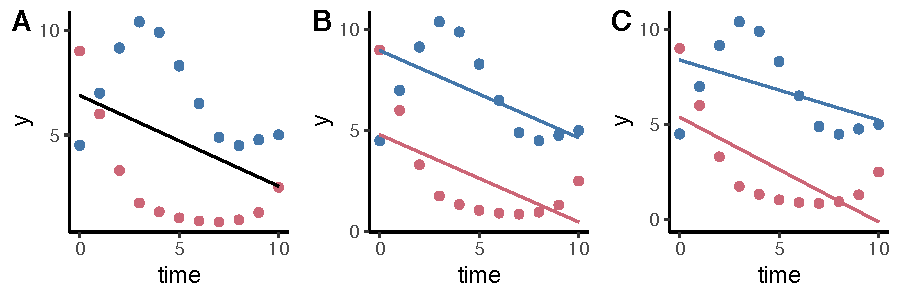
\includegraphics[width=3.9in, left]{Figures/methods/lm_plots.pdf}
    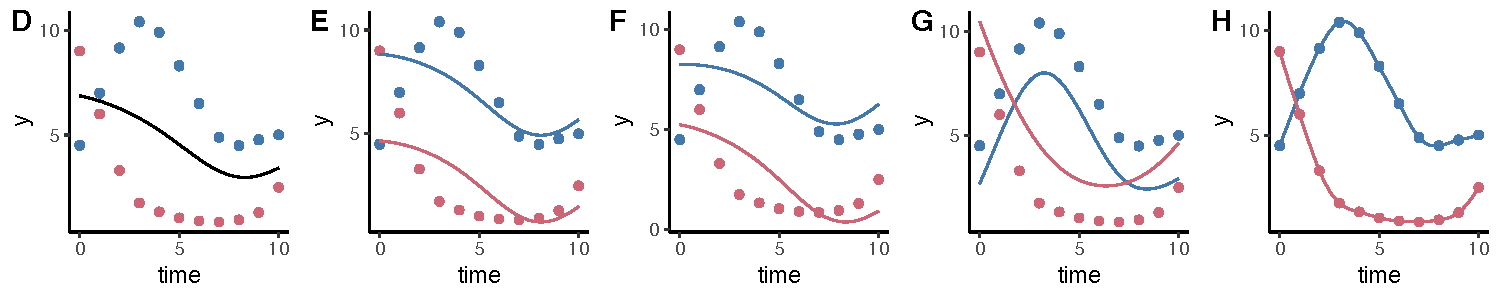
\includegraphics[width = 6.5in]{Figures/methods/gam_plots.pdf}
    \caption[Eight examples of regression models on the same data.]{Eight examples of regression models on the same data. Panels A, B, and C illustrate the capabilities of linear models and panels D, E, F, G, and H illustrate generalized additive models.}
    \label{fig:illustrative_gamms}
\end{figure*}

The lower panels of Figure~\ref{fig:illustrative_gamms} illustrate the effect of GAMs,\footnote{In this series of illustrative plots, I only use fixed effects and no random effects, so the model is simply a generalized additive model (GAM)---with one \textit{m}---rather than a generalized additive \textit{mixed-effects} model (GAMM).} specifically when smooths are added to the model specification. In the simplest model, time is included as a smooth term rather than a parametric term, which allows for a nonlinear best fit line (panel D). As with the linear models, the addition of group as a parametric effect allows for one line per group, though the lines are the same shape and are equidistant from each other at all time points (i.e., they’re parallel; panel E). Likewise, if an interaction term is included between time and grouping, the lines are allowed to have different slopes, but in this case the \textit{shape} of the curves are the same for both groups (panel F). When the group itself is included in the model as a smooth, but without any other parametric effects, the best fit lines for each group are different and resemble the original data, though they are constrained to occupy roughly the same vertical space (panel G). Finally, when group is added as a parametric effect in addition to being a smooth term, the \textit{position} of the lines is allowed to shift vertically, and the best fit line neatly lines up with the data (panel H).

This series of plots illustrates two several points when building a model. First, even the best linear regression model is inadequate to capture a nonlinear pattern in the data. Second, when fitting a GAM, it should include whatever grouping variable of interest as both a parametric effect and a smooth in order to allow to model fit different shapes and positions to the data. Finally, GAMs \textit{can} do an excellent job at fitting the data, but only when properly specified. The models illustrated in panels D--G fail to achieve the potential that a GAM has and are hardly better fits to the data than the linear models represented in panels A--C.

A detailed description of the mechanics of GAMs is out of the scope of this dissertation. For further explanation of generalized additive models (and their mixed-effects counterparts), I refer the reader to the many studies that have implemented these methods, as well as the sources cited within. For a tutorial on GAMMs on linguistic data, see \citet{soskuthy_2017} and \citet{wieling_2018}. Additional studies that implement these models on formant data include \citet{fruehwald_2017}, \citet{renwick_stanley_2020}, \citet{soskuthy_etal_2018}, \citet{warburton_2018}, and \citet{gahl_baayen_2019}. Linguistics studies that use GAMMs on other types of linguistic data include \citet{vanhofwegen_2017_diss}, \citet{kosling_etal_2013}, \citet{tomaschek_etal_2018_phonetics, tomaschek_etal_2018_vanguard}, \citet{strycharczuk_scobbie_2017}, and \citet{mielke_etal_2017}. And for a look at its underlying mathematics, see \citet{faraway_2016} and \citet{wood_2017}.

% TODO (Renwick): Q. some people, like Soskuthy, argue that using difference smooths to pinpoint where two trajectories are significantly different is a risky prospect. Why do you think it's a sound one? [I don't know how to address this because the crux of this dissertation hinges on this being a sound method.]
GAMMs can answer questions about a vowel trajectory that were previously not possible. For example, instead of ``How is the height/backness of \trap different between men and women?'', one could ask, ``How is the trajectory of \trap different between men and women?'' Similarly, one could analyze how a vowel changes shape across time, even if its relative position in the vowel space is the same across generations. Because GAMMs allow for detailed analysis of the full shape of the vowel’s curve (provided a sufficient number of measurements), one could even ask something like ``How does style affect the trajectory of \goose, and at what points along that trajectory is the difference statistically significant?'' Crucially, by analyzing the full trajectory of the vowel, researchers can uncover important linguistic differences that would otherwise not be found when analyzing the midpoints or some other static measure alone.

Why use GAMMs instead of one or more of the existing techniques that study the dynamic nature of vowels? Some studies have implemented techniques such as measuring the vector length, trajectory length, and spectral rate of change \citep{fox_jacewicz_2009, farrington_etal_2018, stanley_renwick_2019_LSA_poster}. Similarly, \citet{morrison_2013} outlines several additional methods that consider various properties of vowel inherent spectral change (the difference between the offset and the offset, the slope of the change, and the direction of change). The utility of these methods cannot be understated since important social patterns have been found to correlate with these measurements. However, they are based on measurements sampled at relatively few time points, and a ``higher resolution'' method can provide a clearer picture of the vowels' behavior. The critical difference boils down to the fact that these techniques allow one to study \textit{properties} of the trajectory while GAMMs allow for the study of the trajectory \textit{itself}. Ultimately, I believe listeners are sensitive to cues in the acoustic signal that are more nuanced than general properties like length and rate of change and that social variation exists in trajectory shape. While GAMMs may not be the ultimate best model to analyze vowel trajectories, they appear to currently be the best technique to uncover this variation.

\section{The implementation of GAMMs in this study}
\label{gamms_in_this_study}

With this background in mind, I now proceed to describe the statistical analyses used for studying the dynamic nature of vowels in the Elsewhere Shift in this sample. To get the most complete picture of the trajectory of a vowel in the F1-F2 space, I analyze their curved trajectories using GAMMs. By examining the model statistics, displaying predicted formant values, and comparing models with different predictor variables, I can identify which factors are influential in the overall shape of the curve. As will be shown hereafter, the use of GAMMs is justified because of the variation in trajectories that would have been overlooked when using single-point measurements alone.

\subsection{Model specificiation}

For each vowel class, I fit a GAMM to the Bark-transformed, normalized values of both F1 and F2 simultaneously in the same model. In most statistical modeling in linguistics, separate models are usually fit to F1 and F2. Sometimes, F1 and F2 are combined into a single measurement, such as the vowel's position along the front diagonal \citep{labov_etal_2013}. Instead, I follow the method used by \citet{gahl_baayen_2019} and \citet{renwick_stanley_2020} and restructure the data such that both F1 and F2 measurements are collapsed into a single \texttt{Hz} variable, which acts as the dependent variable in the model. A new variable, \texttt{formant}, is then included as one of the predictors that indicates whether that measurement is from the first or second formant. Table~\ref{tab:sample_table_wide} illustrates how the data might be structured when constructing a separate model for F1 and F2 and Table~\ref{tab:sample_table_tall} is the restructured data for a pooled model. So, for the main analysis, I fit a GAMM to the Hz measurement for all time points for both formants. This means that the model will take the 11 measurement points from which formants were extracted and essentially ``fill in the gaps'' to allow for a continuous model fit. Because information about what formant the measurement represents is included in the model, separate predictions are made for F1 and F2.

\begin{table}[t!]
    \hspace{\fill}
    \begin{subtable}[t]{0.35\textwidth}
        \centering
        \caption{Sample data, formatted as a ``wide'' table.}
        \liningnums{
            \begin{tabular}{c c c}
                word & F1 & F2\\
                \hline
                A & 1,650 & 600 \\
                B & 1,700 & 615\\
                C & 1,750 & 585
            \end{tabular}
        }

        \label{tab:sample_table_wide}
    \end{subtable}
    \hspace{\fill}
    \begin{subtable}[t]{0.35\textwidth}
        \centering
        \caption{Sample data, formatted as a ``tall'' table.}
        \liningnums{
            \begin{tabular}{ c c r }
                word & formant & {Hz\hspace{1em}}\\
                \hline
                A & F1 & 1,650 \\
                B & F1 & 1,700 \\
                C & F1 & 1,750 \\
                A & F2 &  600 \\
                B & F2 &  615 \\
                C & F2 &  585
            \end{tabular}
        }

        \label{tab:sample_table_tall}
    \end{subtable}
    \hspace{\fill}
    \caption{Two ways of organizing the same set of data. On the left is how FAVE output is formatted. On the right is the reshaped version used for analyses in this study.}
    \label{tab:sample_reshaped_data}
\end{table}

GAMMs are computationally intensive, so I aimed to keep the model specification as simple as possible while accounting for the sources of variation relevant to this study. For language-internal factors, only two variables were included: \texttt{duration} and \texttt{word}. \texttt{Duration} was included as a parametric effect only and it was log-transformed to make it more normally distributed. I include \texttt{duration} (interacting with the sociolinguistic factors as explained below) to allow the model to account for its effect, but it is not considered further in this study. \texttt{Word} was included as a random intercept only, but it was crossed with \texttt{formant} to give it different intercepts for F1 and F2, allowing the predicted trajectory to reposition itself freely in the F1-F2 space. No other phonological factor was included in the models.

Earlier versions of the models included information about previous and following segments. This was done in a host of different ways, such as including voicing and place and manner of articulation as parametric terms and the segment itself as a random effect. However, this model was grossly overspecified. Many combinations of factors were nonsensical for English data (a voiceless velar lateral, for example) and many pairings of previous and following segments were simply unattested due to accidental gaps in the lexicon (e.g. there are no English words with the sequence [\textipa{S\ae S}]). Fortunately, I was justified in removing all phonological factors for two reasons. First, I am not interested in consonantal effects within the defined allophones and I do not anticipate any meaningful variation to occur. But more importantly, whatever variation is captured by including phonological effects in the model is already accounted for (and more!) when word is included as a random effect (Baayen p.c.).\footnote{See \citet[47--48]{gahl_baayen_2019} who adopt the opposite approach and include surrounding segments as random effects rather than word. Either way, limiting the random effects structure is advised so as to avoid overfitting to the data.} So by only including word and duration in the model’s specification, the model was much simpler and had greater statistical and predictive power than an overspecified one with phonological factors also included.
In addition to language-internal factors, I included three variables related to language-external effects: \texttt{speaker}, \texttt{generation}, and \texttt{sex}. As was done with \texttt{word}, \texttt{speaker} was included as a random intercept only and crossed with \texttt{formant} to allow different intercepts per speaker per formant. My original intent was to include \texttt{age} as a continuous variable, rather than \texttt{generation}. I have already shown that language change in Cowlitz County has happened at a nonlinear rate \citep{stanley_2018_pwpl} and given that similar trends have been found in other communities \citep{fruehwald_2017}, I wanted to allow the model to account for a nonlinear rate of change in apparent time, specifically by including \texttt{age} as a smooth. However, this technique resulted in astronomical confidence intervals on the order of tens of thousands of Hz. As I explain in \S\ref{participant_metadata}, the age range in this data is spread over 69 years for just 54 speakers, which is spread thin given that men and women were modeled separately. I took these confidence intervals as a sign that a simpler approach was necessary to get trustworthy results with the current dataset. For this reason, I divided my speakers into generations and used that information in the model.

At the expense of model simplicity, I had theoretical reasons to include interactions between the two sociolinguistic variables (\texttt{generation} and \texttt{sex}). If they were included without any interaction, the model would allow for differences between the sexes and between generations, but the difference between the sexes would be the same in all generations. In other words, this would not be able to account for the possibility of language change happening in men and women at different rates. So, I modeled this interaction between \texttt{generation} and \texttt{sex} and included it both as a parametric effect and a smooth.\footnote{For the smooth, I used the \texttt{gam.check} function in the \texttt{mgcv} package to help determine the number of knots to use for the smooth. The maximum was 10 because I had data from 11 time points. After several tests, it was determined that four knots was sufficient to capture the shape of the curve without being overspecified.} This allowed the model to predict formant trajectories that were different in shape and position in the vowel space for both sexes in all four generations. However, to allow for independent curves for both formants in each of these combinations of factors, I actually had to create a three-way interaction between \texttt{generation}, \texttt{sex}, and \texttt{formant}. For example, if an observation is an F1 measurement from a baby boomer–aged woman, that information would be expressed as the string \texttt{F1\_F\_boomer} in the data. This interaction term had 16 such levels, representing the 16 combinations of \texttt{formant}, \texttt{sex}, and \texttt{generation}. Again, this comes at the expense of model simplicity, but I felt that it was important to allow all of these factors to vary freely.

Finally, the model controlled for autocorrelation between the residuals by including an AR1 residual error model. To do this, a model is fit without autocorrelation which is then used to calculate a value called rho. The rho value is then used in the calculations for the AR correlation in a second version of the model. (This original model is then discarded.) The following code was used to fit these models.\footnote{The crucial elements of this code block, which give the model the flexibility illustrated in Panel H of Figure~\ref{fig:illustrative_gamms} above, are the second and third lines.}

\begin{verbatim}
1  mdl_seed <- mgcv::bam(anae_barks ~
2                 formant_sex_gen +
3                 s(percent, by = formant_sex_gen, k = 4) +
4                 log(dur) * formant_sex_gen +
5                 s(word, formant, bs = "re") +
6                 s(speaker, formant, bs = "re"),
7              data = df, discrete = TRUE)
8  rho <- start_value_rho(mdl_seed)
9  mdl <- update(mdl_seed, rho = rho, AR.start = df$start_event)
\end{verbatim}


Using this template, identical models were then fit to each vowel class in this study. It took a little over two hours to run all models on my computer.

\subsection{Interpreting the GAMMs' output}
\label{sec:interpretation_of_gamms}

Determining whether a variable is significant\footnote{Around the time this draft was completed, \textit{The American Statistician} published a special issue called ``Statistical Inference in the 21st Century: A World Beyond \textit{p}~$<$~0.05''. This collection of 43 articles urges researchers to abandon traditional ideas of statistical significance: ``it is time to stop using the term `statistically significant entirely'' \citep[2]{wasserstein_etal_2019}. Though I still rely on confidence intervals in this study, which are ultimately derived from ``statistically significant`` \textit{p}-values, I do interpret these models with some care. Ultimately, I strived to heed to their advice: ``Accept uncertainty. Be thoughtful, open, and modest'' (ibid.).} in a GAMM is not as it is with other types of models. Because the three-way interaction variable is contained in the models both as a parametric term and as a smooth, it is not always straightforward to determine statistical significance from the model summary alone, particularly when the goal is to determine the significance of just one of those social factors. In particular, because of the way these interactions were implemented (i.e. a forced interaction by combining the constituent variables), lower-order terms were not included in the model.

For example, consider a hypothetical situation in which speaker sex was not relevant for some variable for this community. In a mixed-effects linear regression model fit with the \texttt{lmer} function in the \texttt{lme4} package \citep{bates_etal_2015_lme4}, I would create interaction terms by crossing the variables in the model formula itself (i.e. \texttt{sex * generation}). In the model summary, not only would I see the effect of this interaction, I would also see the effect of the factors themselves. If sex were not significant, neither interaction of \texttt{sex * generation} nor \texttt{sex} as an independent variable on its own would be statistically significant, but \texttt{generation} by itself would be. The model summary would lead me to conclude that \texttt{sex} may be removed from the model to create a better fit to the data. Unfortunately, such output is not possible with the current implementation of the \texttt{bam} function in \texttt{mgcv} \citep{wood_2017} so testing the effect of one of the variables in the interaction is not possible with the model's output alone.

Fortunately, the significance of a variable can still be tested by fitting two models---one with the variable (the ``full'' model) and one without (the ``base'' model)---and comparing their fit to the data. If the inclusion of that predictor improves model enough to justify the extra complexity, it is considered a significant predictor. (This method is also used to test the significance of predictors in linear regression or linear mixed-effects models.)

In all cases though, \texttt{formant} was retained in the ``base'' models because I always expect significant differences between F1 and F2 regardless of the social factors in the model. These comparisons were made using the \texttt{compareML} function in the \texttt{itsadug} package \citep{van_rij_etal_2017_itsadug}.\footnote{Note that comparison of models that include the AR1 model make the AIC scores unreliable, but the significance tests can still be trusted (Renwick, p.c.). } For all vowels, the model comparisons suggest that the inclusion of sex and generation significantly improve the model fit (Appendix~\ref{appendix:model_comarisons}, so their output will not be described in much detail in the results chapters.

%However, because the predictors were included in the model only as part of a three-way interaction term, the comparison is not simply between a full and base model. Instead, all possible subsets of the three-way interaction are created and separate models are fit with those lower-order interactions (Figure~\ref{fig:model_nesting}).

%\begin{figure}
%    \centering
%    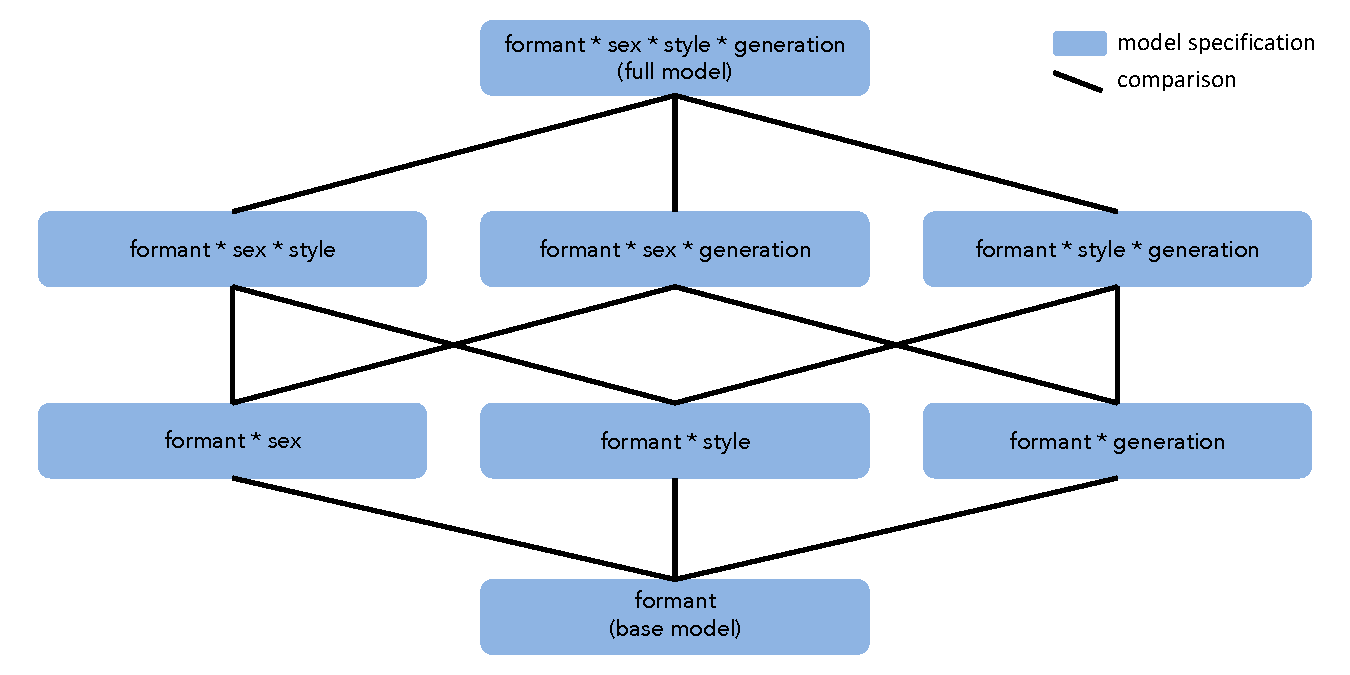
\includegraphics[width=\textwidth]{Figures/methods/subset.pdf}
%    \caption[A visualization of the models created for each vowel.]{A visualization of the models created for each vowel. Boxes represent models and lines connecting them represent one comparison test that was implemented. Incidentally, parallel lines indicate the addition of the same variable: all vertical lines connect models that differ only by the addition or removal of style and test for its significance, diagonal lines from bottom left to top right test for generation and diagonal lines from bottom right to top left test for sex. Theoretically, if a variable has absolutely zero correlation with the depedent variable, the model comparison tests that the parallel lines represent would not be statistically significant.}
%    \label{fig:model_nesting}
%\end{figure}

%Imagine again a scenario in which style is not a significant factor in the data, but it is still included in the four-way interaction. This full model (labeled A in Figure~\ref{fig:model_nesting}) is compared against a model that does not account for style whatsoever with only a three-way interaction between formant, sex, and generation are included (B). In the model comparison (line a-b), the simpler model without style (B) would be considered the better fit to the data because it accounts for the same amount of variance with a less complex model specification (A). However, in this scenario, imagine that generation is a significant predictor: a model that contains only a three-way interaction between formant, sex, and style (C) would perform worse in comparison (a-c) to the full model (A) because the larger model accounts for much more of the variation. This is seen in the output of the model comparison and is justification for including generation in the model. But, as additional support that style is not a significant predictor, the model with the three-way interaction of formant, sex, and style (C) would also be a worse fit than one with a two-way interaction between formant and sex (neither style or generation are in this smaller model; D; c-d) because whatever variance the three-way interaction can account for, the two-way interaction can also explain it with less complexity.

\section{Visualizing the GAMMs' predicted values}
\label{sec:visualizing_gamms}

While these model comparisons helps determine a variable’s significance in the model, it does not help the analyst understand what kind of effect it has on the shape of the curve. And because of the non-linear effect the variables have on the predicted values, the coefficients of predictors by themselves are largely uninterpretable by any analyst because they do not indicate anything about the shape of the curve. Therefore, a visualization of the predicted values is provided to clarify how the model was fit to the data. They also provide a useful way to show trajectory data. The authors of the \textit{Atlas of North American English} describe the difficulty in visualizing trajectory data:
\begin{quote}
    ``While it is easy to plot an array of sequential measurements of a single vowel, plotting 300 such trajectories for a single speaker would obscure any pattern and preclude the goal of describing the vowel systems of North America'' \citep[38]{labov_ash_boberg_2006_anae}.
\end{quote}
Essentially, a visualization of all the raw trajectory data in the F1-F2 space looks like a bowl of spaghetti and the patterns are impossible to discern. The predicted values from a GAMM consolidate vowel tokens and groups of speakers into a single line. Therefore, visualizations of these predicted values allow for a consolidated view of the data, relatively free from the noise and messiness inherent in data extracted using automatic means.

I therefore present model visualizations in three primary types of multi-panel plots: F1-F2 plots, spectrogram-like plots, and difference smooths.

\subsection{F1-F2 plots}

\begin{figure*}[tb!]
    \centering
    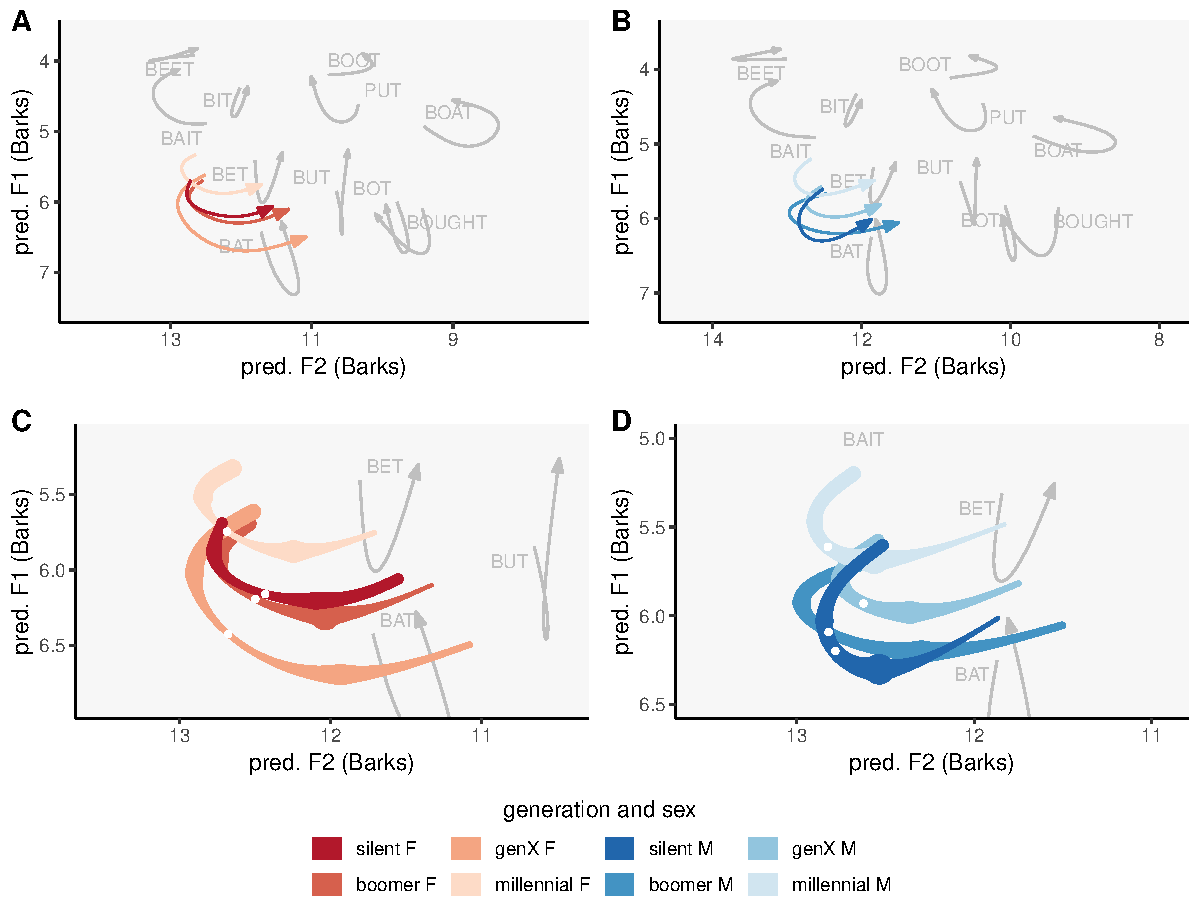
\includegraphics[width = 6.5in]{Figures/BAN/BAN_four_panel_plot.pdf}
    \caption[A sample four-panel plot used in this dissertation.]{A sample four-panel plot used in this dissertation. This shows the \ban vowel and is explained in more detail in \S\ref{BAN}.}
    \label{fig:sample_four_panel_plot}
\end{figure*}

In the results chapters, I present model visualizations in a series of four-panel plots, each displaying different views of the predicted values in the F1-F2 space. Figure~\ref{fig:sample_four_panel_plot}, taken from \S\ref{BAN}, is an example of such a plot. All images display a set of curves in color, representing the predicted values for the vowel in question. Another set of curves is underlayed in gray and represent the predicted values for all vowels\footnote{The underlaid trajectories represent elsewhere allophones of the other vowels too. Prelateral and prerhotic tokens are not included when calculating these trajectories. Furthermore, post-cororanl tokens of \goose and \goat were excluded to form the \boot and \boat allophones.} in the entire community as a point of reference. All plots are in the Bark-transformed, normalized F1-F2 vowel space. Panels A and B (on the top) offer a ``zoomed out'' view, allowing the viewer to examine the trajectories in relation to other vowels and to see their position in the vowel space. Panels C and D are ``zoomed in'' to facilitate viewing the shapes of the curves themselves. The data presented in the left two panels (A and C) are identical and always show the women’s data in shades of red. Likewise, the two panels on the right (B and D) display the men’s data, which is identical between the two panels, in shades of blue. On the top two plots, a small arrow has been placed on the offset of the vowels to indicate the direction of movement. The thickness of the lines in the bottom two panels corresponds to the rate of change, with thicker portions representing little movement, and narrow portions showing fast change, as if they were drawn with a quill pen.\footnote{For the curious, I am not aware of a way to get a continuous change in line thickness in \texttt{ggplot2}. I pulled off this effect by extracting predicted values at 501 equally spaced intervals along the vowels' duration (0.2\% intervals) and plotted them as points. The size of the circles reflects the euclidean distance from the previous point. Because so many points are all plotted so closely, the effect is a smooth line that changes width. I credit \citet{fruehwald_2017_gamm} for the idea for these plots.} Furthermore, on the bottom two plots, a small white dot has been placed on the midpoint of the vowel, illustrating what information would have been gleaned had only single-point measurements been used in this study and to facilitate comparison with previous studies.

These plots contain a wealth of information about the predicted values of these GAMMs. Their interpretation is facilitated by the fact that each set of four-panel plots is formatted and sized identically throughout this dissertation,\footnote{To ensure all the plots are identically formatted, I wrote a custom R function that takes in a GAMM and produces the full four-panel image.} so once the reader has learned to read one, they will be able to read them all. The only thing that changes from plot to plot is the data being displayed, and the axes of the bottom plots (the axes on the top two are fixed).


\subsection{Spectrogram-like plots}

\begin{figure*}[tb!]
	\centering
	%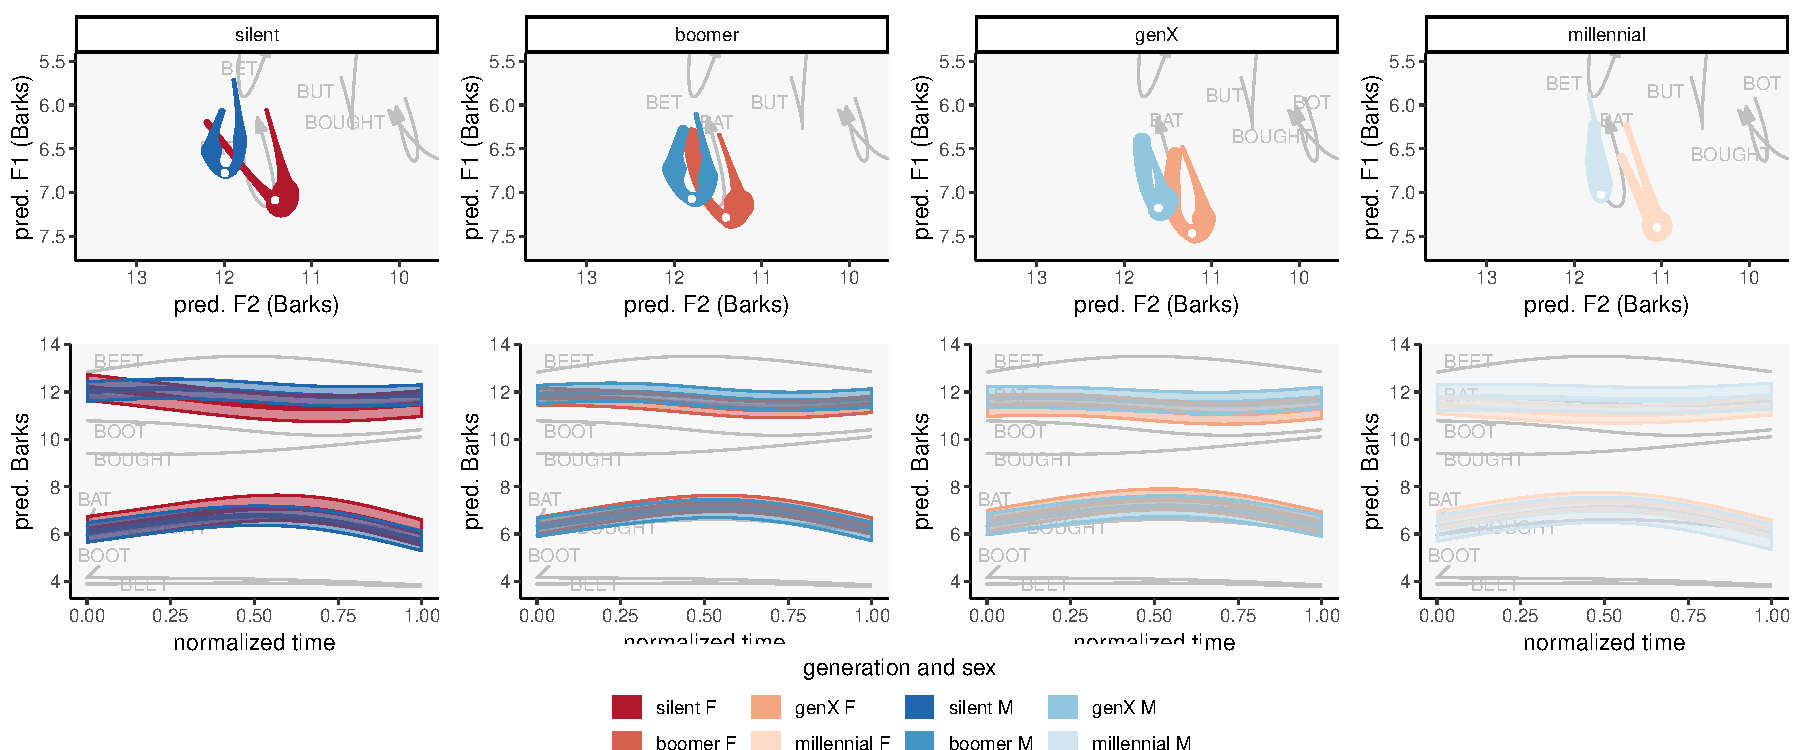
\includegraphics[angle = 90, origin = c, height = 6in]{Figures/BAT/BAT_sex_panel_plot_wide.pdf}
  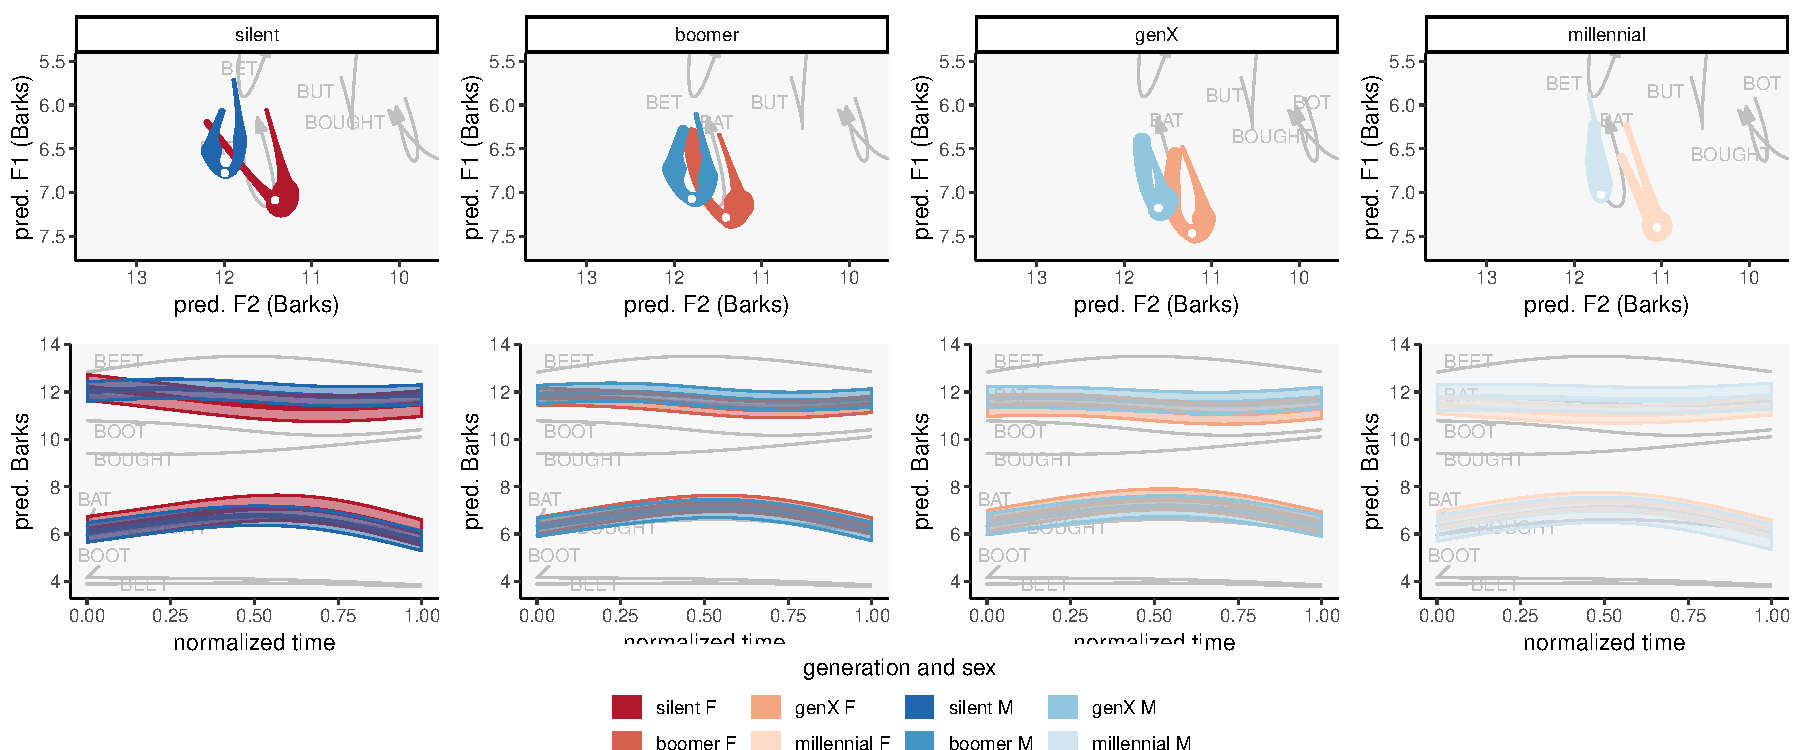
\includegraphics[width = 6.5in]{Figures/BAT/BAT_sex_panel_plot_wide.pdf}
	\caption[A sample eight-panel plot used in this dissertation.]{A sample eight-panel plot used in this dissertation. This shows the \ban vowel and is explained in more detail in \S\ref{BAN}.}
	\label{fig:sample_spectrogram_plot}
\end{figure*}

As an alternative view of the data, I also present the formant trajectories in plots that are reminiscent of spectrograms. By this, I mean that time is along the \textit{x}-axis and formant frequency (in Barks) is along the \textit{y}-axis. These should be familiar to those comfortable with viewing spectrograms in programs such as Praat.

Figure~\ref{fig:sample_spectrogram_plot} is an example of a series of plots that uses these spectrograms. In this layout, the four generations are split up, with the oldest generation on the left and the youngest generation on the right. The top four panels show predicted formant values in the F1-F2 space, just as they are displayed in the other F1-F2 plots, with the difference being that men and women are plotted together, but only from one generation.

Underneath these plots are the spectrograms. The \textit{x}-axis, going from left to right, represents normalized time, with the vowel onset on the left edge and the offset on the right edge. The lower two bands represent F1 and the upper two represent F2, with women in shades of red and men in shades of blue. For ease of interpretation between the different plots, the colors and shades are identical with those in four-panel plots described in the previous section.\footnote{It was difficult to find four shades that worked harmoneously together while being able to stand out against a white background. Consequently, the colors used for the Millennials are admittedly a little too faint. Unfortunately, due to COVID-19, I was unable to return to campus to retrive my data, meaning I could not rerun the models and reproduce the visualizations in time for this dissertation to be submitted.} Like the F1-F2 plots, faint gray lines are underlaid to show what the predicted formant trajectories were for four corner vowels, to show the extremes in formant frequencies.

\subsection{Difference smooths}

Finally, the last type of visualization used in this dissertation are a special kind of output called \textit{difference smooths}. Since these are only used in Appendix~\ref{appendix:difference_smooths}, a detailed description of how to interpret those plots is found there.

\subsection{A typology of formant curves}

Because relatively few sociolinguistic studies have analyzed formant curves in the F1-F2 space in depth, we lack the terminology needed to describe the shape of these curves. In this section, I propose five types of formant curves, which are illustrated in an idealized form in Figure~\ref{fig:curve_types}. The top panels represent what these curves would look like in the F1-F2 space while the bottom panels show what the formant movement would look like in a spectrogram.

\begin{enumerate}
  \item \textit{The Line}---This is the most basic formant shape, the onset is in one point in the vowel space, the onset is in another, and the trajectory connects the two in a straight line. When oriented horizontally as in Figure~\ref{fig:curve_types}, there is no formant movemement in F1. Note that an analysis that extracts formant measurements at only two timepoints will result in all vowels being of this type, which may be a simplication of a more complex underlying curve. If however additional measurements are taken and the trajetory is still a line, then it may be said that that vowel has this shape.
  \item \textit{Bounce}---In the F1-F2 space, the Bounce appears to move from one point to another and then back in a straight line. When oriented vertically as it is in Figure~\ref{fig:curve_types}, F2 is constant throughout the duration of the vowel. F1, meanwhile, ascends and then descends.\footnote{It is probably of little consequence whether the rate of change in F1 is constant. The F1-F2 plot would look the same regardless (unless rate of change is incorporated into the visual), though a spectrogram would reveal a more curved arc rather than a jagged point.} The point of inflection in F1 is clear and would presumably be the target of the vowel. An analysis that extracts measurements at only three timepoints may find a Bounce in all vowels, so data from additional timepoints are necessary to identify whether a trajectory is truly a Bounce.
  \item \textit{The V}---The V is similar to the Bounce, only there is (presumably constant) movement in F2 over the course of the vowel's duration.\footnote{Obviously the Bounce and the V represent points along a continuum and in some cases a curve will fall somewhere between the two.} The target is still clearly defined as the point of inflection in F1. The V and Bounce can each be described as ``pointy'' trajectory shapes, reflecting the abrupt reversal in F1 and clear point of inflection in the F1-F2 space. Like the Bounce though, the V will be common, if not the norm, in a three-point analysis and only after extracting measurements from more timepoints will an underlying V shape be revealed.
  \item \textit{The U}---Adding complexity to the V, the U introduces a smoother formant movement than the two ``pointy'' shapes described above. In this example, F2 still descends at a constant rate and while F1 does ascend and descend like the Point and the V, it does so more smoothly than in the V. In the F1-F2 space, the U still has a target, though it is less clearly identifiable; there is no steady state in U-shaped trajectories.
  \item \textit{The Bowl}---Like the other shapes, F1 rises and falls in the Bowl trajectory shape, but unlike the other types, there is no clear inflection point. In both the F1-F2 plot and the spectrogram, there is no easily identifiable target. In the spectrogram, the rate at which F1 increases decelerates to a point where there is almost a flat formant trajectory for a brief time,\footnote{Similarly, a bowl is flat on the bottom so it can rest on a table.} after which F1 slow begins to lower again, picking up speed towards the ends of the vowel's duration. In the Bowl, the point of inflection in F1 is somewhat arbitrary and, as suggested in the F1-F2 plot, it is unclear if that point would actually represent a target. Instead, the F1-F2 suggests that there are two targets in a Bowl, one corresponding to each of its ``corners'', though it is unclear what the acoustic correlates of these corners might be (or indeed how to identify them in the spectrogram).
\end{enumerate}

\begin{figure*}[tb!]
    \centering
    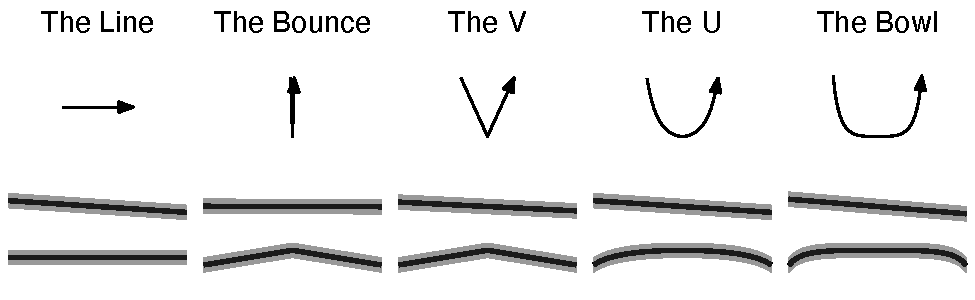
\includegraphics[width = 6.5in]{Figures/other_figures/traj_shapes.pdf}
    \caption{Five types of formant curves}
    \label{fig:curve_types}
\end{figure*}

These descriptions, especially the particulars of the formant movements, are based on the idealized versions of these trajectories displayed in Figure~\ref{fig:curve_types}. In reality, the data will be messier. For example, any of these trajectories can be rotated to an arbitrary angle. If the formants swap roles (e.g., F1 changes at a constant rate while F2 has a curved shape in the U), then the curve will appear sideways in the F1-F2 plot. If F2 lowers gradually rather than raises, the direction of movement will go the opposite way (and visually, the arrow will be on the other end), creating ingliding or offgliding variants. In this study, if a trajectory has an offset with a lower F2 than the onset (as in Figure~\ref{fig:curve_types}, depicted visually with the arrow on the right), I often call it \textit{right-hooking} (or ingliding since I deal primarily with front vowels). For trajectories that go the opposite way, I call them \textit{left-hooking}.

\begin{figure*}[tb!]
    \centering
    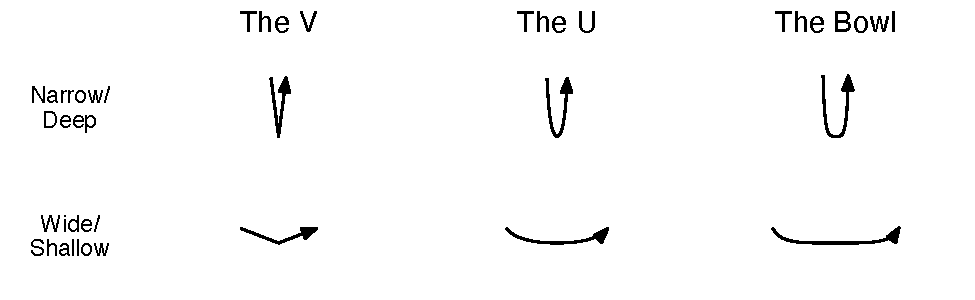
\includegraphics[width = 6.5in]{Figures/other_figures/traj_shapes_mod.pdf}
    \caption{Modified versions of the formant types.}
    \label{fig:curve_types_mod}
\end{figure*}

It may be helpful to modify the terms with adjectives to describe the amount of change in one formant relative to the other (\ref{fig:curve_types_mod}). For example, a Bounce is essentially a very \textit{narrow} V, meaning that F1 changes much more relative to F2. Alternatively, a very \textit{wide} V would have much more change in F2 than in F1 and may even approach the Line. One may also find narrow and wide U and Bowl shapes as well. Alternatively, the terms \textit{deep} and \textit{shallow} may be used, perhaps synonymously with \textit{wide} and \textit{narrow}. To be clear, the Bowl is not simply a wide U because the Bowl has two inflection points and the U has only one; however, a narrow Bowl may be simply described as a U because there is likely little need of describing two very close inflection points.

The point is that these labels are primarily descriptive and are not necessarily meant to represent differences in how formant trajectories are stored at the cognitive level.\footnote{However, it could be tested experimentally whether listeners discern differences between these formant shapes.} The difference between a Bounce and a narrow V and between a U and a Bowl can be subjective. The difference between a Line and a very shallow V or U is not clear either. For now, I present these terms to ease descriptions of formant trajectories in this study.

Finally, these terms were developed based on the data analyzed in this dissertation and, perhaps more importantly, upon the analysis used. Since these GAMMs fit curves with only 4 knots, there can only be so much wiggliess in the resulting shape. A triphthong likely exhibits additional complexity that four knots (and these five descriptive terms) cannot handle. Therefore, while these terms may be useful to other researchers who study formant movement, it is not a closed class of labels.







\section{How to identify and quantify vowel shift}
\label{how_shifting_is_measured}

After the GAMMs have been fit to the data, the final step in the analysis is to actually determine whether the vowels have shifted in apparent time. In this section, I describe methods used to determine whether vowels have shifted and weigh their pros and cons. I ultimately choose to simply compare younger generations to older generations in this community.

\subsection{Method I: Relative position from an anchor vowel}

In general, in order to show that vowels change is to do so in relation to some stable or anchor vowel \citep[103--104]{dipaolo_etal_2011}. For example, the height of \trap is often compared against that of \lot \citep[20]{thomas_2001}. Lowering of \bit is sometimes determined by comparing its F1 to \face's F1 (\citealt[44]{kennedy_grama_2012}, \citealt[97]{bowie_2017_pads}). In a large sample including Canadians and Americans, \citet{boberg_2019} finds that \kit has shifted lower than \face and that \trap is further back than \goose and is close to the nucleus of \mouth. These are useful measurements, especially considering that vowel’s canonical positions are generally known.

However, in Western American English, all vowels are undergoing a change of some sort: \kit, \dress, and \trap are lowering and/or retracting as part of the Elsewhere Shift, the merged \lot-\thought vowel is raising and backing, and all other back vowels are fronting. Of the remaining vowels, \fleece is lowering and retracting in California \citep{donofrio_etal_2019} and \face is more monophthongal in Washington than elsewhere in the West \citep{wassink_2015}, so their usefulness as reference points would vary across the West. Thus, a description of one vowel in relation to another is potentially problematic in Western American English.

Nevertheless, the stable position of \fleece in other areas is perhaps the motivation for the development of a unitary measure of the Elsewhere Shift: the \textit{Short Front Vowel Shift Index} \citep{boberg_2019}.\footnote{This method is also used by the various authors in the recent volume on the Elsewhere Shift \citep{becker_2019_pads}.} This index is calculated as the average Cartesian distances between \fleece-\kit, \fleece-\dress, and \fleece-\trap, using mean values for each vowel. A similar method was adopted by \citet{holland_2019}, \citet{pratt_donofrio_2017}, and to some extent \citet{podesva_etal_2015}. One benefit of this multivariate measure is that it gets away from a strict separation of the F1 and F2 dimensions \citep{becker_2019_pads}. However, a measure that reduces the shifts of three vowels down to a single number may make sense for versions of the Elsewhere Shift in which the three are retracting in parallel at the same time. But if the vowels are more independent, such as what is found in this study, this single number may not be the most appropriate way to measure the Elsewhere Shift.

% TODO Read Kendall & Fridland 2017 (LVC) for measures from BOT. Also, Swan (2019).

\subsection{Method II: Comparison against \textit{ANAE} benchmarks}

What is needed is some stable reference value to compare formant measurements against. These reference values would presumably measure what a conservative or innovative vowel might be, and measurements in relation to these benchmarks would determine the degree of shifting. The closest thing to these benchmarks are the values used in maps of the \textit{Atlas of North American English}. For example, in a map that illustrates the Canadian Shift (Map 15.4, page 219), speakers are coded as either having the Canadian Shift or not. Given their average measurements per vowel, if a speaker’s F1 for \dress was greater than 660, F2 for \trap was less than 1825, and F2 for \lot was less than 1275, than they were coded has having the Canadian Shift. Speakers that did not satisfy all three of these requirements were considered to not have the shift. This way of determining the presence of the shift was useful in the construction of that map, which showed a high degree of homogeneity among Canadian speakers.

These values have since been used as benchmarks to determine whether \lot, \trap, or \dress are retracted or lowered. For example, \citet[44]{kennedy_grama_2012} state that ``subjects meet the definition of the Canadian shift if they have (1) F1 of \dress greater than 650 Hz, (2) F2 of \trap less than 1825 Hz, and (3) F2 of \lot less than 1275 Hz.'' Similarly, \citeauthor{becker_etal_2016_pads} use these values and state that ``[v]owels which cross these cut-off points are considered shifted'' \citeyearpar[113]{becker_etal_2016_pads}. Similar methods are also adopted in studies on the Elsewhere Shift in New Mexico \citep{brumbaugh_koops_2017_pads} and Utah \citet{bowie_2017_pads}. Thus, it appears that though all vowels are shifting in the West, these benchmarks satisfy the need for stable, reference values to measure the Elsewhere Shift.

However, it does not appear that these numbers were intended to be used for that purpose. For one, these numbers only appear in the \textit{ANAE} maps' legends and are not mentioned in the text. Furthermore, they are different from map to map: Map 11.7 (page 132), which also shows the Canadian Shift, has the F1 threshold for \dress as 660 Hz instead of 650 Hz. And though the cutoff for a shifted \trap was 1825 Hz, the mean F2 for Canadian speakers’ realization of \trap was 1725 Hz. These are admittedly small differences, but they illustrate that the cutoff values are not absolutely fixed. If these numbers were intended to be important benchmarks for determining degree of shifting, should they be not consistent from map to map, perhaps presented in a table in the text itself, and described in detail as to how and why those particular values were determined?

Instead, it appears that these numbers were used solely for the purpose of creating the isoglosses for the maps. F1 and F2 are continuous measurements, so it is somewhat meaningless to divide the range of values into ``shifted'' or ``not shifted.'' Nevertheless, this binary split was necessary because the method used for determining isoglosses was an iterative process which sought to maximize either the homogeneity of speakers within a determined region or the proportion of speakers that have a particular linguistic feature. After an isogloss is drawn, it was evaluated and altered until it converged on an optimal dialect boundary. As part of this altering process, the cutoff value for determining the presence or absence of a linguistic feature could be modified if it resulted in a better fitting isogloss: ``one may adjust this value to maximize either homogeneity or consistency'' \citep[43]{labov_ash_boberg_2006_anae}. Thus, the benchmarks were allowed to vary from map to map (as in Map 11.7 and Map 15.4) to produce cleaner isoglosses. It does not appear to be the case that these numbers are meant to be absolute cutoff values that determine presence or absence of a vowel shift in a theoretical way. Instead, it appears then that these arbitrary benchmarks were calculated to be the best for maximizing homogeneity and drawing an isogloss around the most consistent group of speakers within that dataset.

Therefore, treating these values as strict benchmarks can be potentially problematic when speakers who are expected to shift do not meet the qualifications. \citeauthor{kennedy_grama_2012} find that their sample of California-based speakers passed the threshold for \dress lowering and \trap retraction but that they ``cluster around'' the threshold for \lot retraction \citeyearpar[49]{kennedy_grama_2012}. This is their primary support for the Canadian Shift and California Shift being independent processes and for the low back merger not necessarily being the trigger of \trap retraction. Furthermore, the arbitrary threshold divided their speakers into those with vowels similar to those in the Canadian Shift and the ``remaining subjects [who] are somewhat of a mystery'' \citeyearpar[51]{kennedy_grama_2012}. Treating these benchmarks as general guidelines instead of absolute cutoffs may reduce the need for dividing a somewhat homogeneous cluster into two groups.

Finally, \citet{dinkin_2018} points out that in order to appropriately apply these benchmarks to a new dataset, the data must be normalized using the same procedure as the one used in the \textit{Atlas of North American English}. Because the units of these benchmarks are in Hz, it is not immediately apparent that the data are normalized and that similar techniques are required to apply a meaningful interpretation onto a new dataset. With what is probably the most popular normalization procedure in sociolinguistics, the \citet{lobanov_1971} transformation converts F1 and F2 values into z-scores (i.e. number of standard deviations from the mean values). For researchers who use FAVE, which may be the most common method for formant extraction in North American sociolingustics, these z-scores are then rescaled so that F1 has a mean of 650 Hz with a standard deviation of 150 Hz and F2 has a mean of 1700 Hz and a standard deviation of 420 Hz. Thus, the methods used by FAVE and by the \textit{Atlas of North American English} produce values that are Hz-like and are in the expected ranges. But comparing results from one method with another (or against raw measurements) is like comparing apples to oranges. \citet{dinkin_2018} explains that the differences may seem superficial, but a reanalysis of his data shows that the F1 of some speakers’ \trap vowel is below the \textit{ANAE} benchmark of 1825 Hz when using one method and above it when using the other. In other words, conclusions drawn about the degree of shifting can entirely depend on using the proper normalization procedure when comparing to the \textit{ANAE} benchmarks.

\subsection{How shifting is measured in this study}

In this section, I have discussed the need for some sort of stable reference values to measure the degree of shifting and have critiqued the use of the \textit{ANAE} benchmarks to serve this purpose. To my knowledge, there are no other reference values that have been used to show whether the front lax vowels are shifting. To complicate matters even more, how should such a benchmark be treated when vowel dynamics are considered? Does the entire trajectory need to be past the cutoff value or is just one measurement sufficient? If some proportion of the trajectory should be past the benchmark, how does one determine the amount? To my knowledge, there really is no agreed-upon way to objectively measure the degree of shifting across studies.

For now, the best solution---and the method that I use in this study---is to focus on one vowel and compare the realizations used by two different groups. In other words, the most effective way for analyzing shift in apparent time is by comparing older people to younger people in the same community \citep{boberg_2005, cardoso_etal_2016_pads, holland_brandenburg_2017_pads, hall_lew_etal_2017}. Comparing pronunciations by different genders and ethnicities \citep{brumbaugh_koops_2017_pads} can also help determine the relative amount of shifting between groups. When visualizing the vowel space, it is also be ideal for other vowels for these groups of speakers to also be plotted, partially as reference values, but also to give an idea of the degree of shifting, with the understanding that these reference vowels may also be changing in time. This method for gauging how much shifting is occurring is not entirely satisfactory because it makes it impossible to determine whether one community is more shifted than another. Nevertheless, this is the method used in this study and I leave it to future work for determining a more objective way for comparing the shift across studies.

\section{Hardware and software}
\label{r_packages}

Data processing and analysis for this study was done using version 3.5.1 of R programming language \citep{r_2018} using version 1.1.463 of the RStudio software. In addition to the many functions that come with the standard distribution of R, I relied heavily on these packages:

\begin{itemize}
    \item The bulk of data processing, transformation, and cleanup was done using the various packages in the \texttt{tidyverse} \citep{wickham_2017_tidyverse} including \texttt{readr} \citep{wickham_etal_2018_readr}, \texttt{readxl} \citep{wickham_bryan_2019_readxl}, \texttt{dplyr} \citep{wickham_etal_2019_dplyr}, \texttt{tidyr} \citep{wickham_henry_2018_tidyr}, \texttt{stringr} \citep{wickham_2019_stringr}, and \texttt{forcats} \citep{wickham_2019_forcats}.
    \item To manage the many models in this study, I used \texttt{modelr} \citep{wickham_2019_modelr} and \texttt{broom} \citep{robinson_hayes_2018_broom}.
    \item The models themselves were run using \texttt{mgcv} \citep{wood_2017} and the predicted values were extracted using \texttt{itsadug} \citep{van_rij_etal_2017_itsadug}.
    \item All visualizations were done in \texttt{ggplot2} \citep{wickham_2016_ggplot2} with the help of \texttt{ggrepel} \citep{slowikowsky_2018_ggrepel} for vowel labels. They were combined into the four-panel plots using \texttt{cowplot} \citep{wilke_2019_cowplot}.
    \item All non-gray colors in the visualizations are from Paul Tol's \citeyearpar{tol_2012} color schemes, accessed via \texttt{ggthemes} \citep{arnold_2018_ggthemes}.
\end{itemize}
The hardware was an early 2014 model MacBook Air running macOS 10.14 (Mojave). The bulk of processing was done in late 2018.

% Praat
% QGIS plus data sources
% LaTeX
